%%%%%%%%%%%%%%%%%%%%%%%%%%%%%%%%%%%%%%%%%
% Doctoral Thesis 
% LaTeX Template
% Version 2.5 (27/8/17)
%
% This template was downloaded from:
% http://www.LaTeXTemplates.com
%
% Version 2.x major modifications by:
% Vel (vel@latextemplates.com)
%
% This template is based on a template by:
% Steve Gunn (http://users.ecs.soton.ac.uk/srg/softwaretools/document/templates/)
% Sunil Patel (http://www.sunilpatel.co.uk/thesis-template/)
%
% Template license:
% CC BY-NC-SA 3.0 (http://creativecommons.org/licenses/by-nc-sa/3.0/)
%
%%%%%%%%%%%%%%%%%%%%%%%%%%%%%%%%%%%%%%%%%

%----------------------------------------------------------------------------------------
%	PACKAGES AND OTHER DOCUMENT CONFIGURATIONS
%----------------------------------------------------------------------------------------

\documentclass[
11pt, % The default document font size, options: 10pt, 11pt, 12pt
%oneside, % Two side (alternating margins) for binding by default, uncomment to switch to one side
english, % ngerman for German
singlespacing, % Single line spacing, alternatives: onehalfspacing or doublespacing
%draft, % Uncomment to enable draft mode (no pictures, no links, overfull hboxes indicated)
%nolistspacing, % If the document is onehalfspacing or doublespacing, uncomment this to set spacing in lists to single
%liststotoc, % Uncomment to add the list of figures/tables/etc to the table of contents
%toctotoc, % Uncomment to add the main table of contents to the table of contents
%parskip, % Uncomment to add space between paragraphs
%nohyperref, % Uncomment to not load the hyperref package
headsepline, % Uncomment to get a line under the header
%chapterinoneline, % Uncomment to place the chapter title next to the number on one line
%consistentlayout, % Uncomment to change the layout of the declaration, abstract and acknowledgements pages to match the default layout
]{MastersDoctoralThesis} % The class file specifying the document structure

\usepackage{amsmath}
\usepackage{float}
\usepackage[utf8]{inputenc} % Required for inputting international characters
\usepackage[T1]{fontenc} % Output font encoding for international characters

\usepackage{mathpazo} % Use the Palatino font by default

\usepackage[backend=bibtex,style=authoryear,natbib=true]{biblatex} % Use the bibtex backend with the authoryear citation style (which resembles APA)

\usepackage{xcolor}
\usepackage{listings}

\addbibresource{example.bib} % The filename of the bibliography

\usepackage[autostyle=true]{csquotes} % Required to generate language-dependent quotes in the bibliography

%----------------------------------------------------------------------------------------
%	MARGIN SETTINGS
%----------------------------------------------------------------------------------------

\geometry{
	paper=a4paper, % Change to letterpaper for US letter
	inner=2.5cm, % Inner margin
	outer=3.8cm, % Outer margin
	bindingoffset=.5cm, % Binding offset
	top=1.5cm, % Top margin
	bottom=1.5cm, % Bottom margin
	%showframe, % Uncomment to show how the type block is set on the page
}

%----------------------------------------------------------------------------------------
%	THESIS INFORMATION
%----------------------------------------------------------------------------------------

\thesistitle{A Language of Polynomials} % Your thesis title, this is used in the title and abstract, print it elsewhere with \ttitle
\supervisor{Dr. xxx \textsc{xxx}} % Your supervisor's name, this is used in the title page, print it elsewhere with \supname
\examiner{} % Your examiner's name, this is not currently used anywhere in the template, print it elsewhere with \examname
\degree{Doctor of Philosophy} % Your degree name, this is used in the title page and abstract, print it elsewhere with \degreename
\author{Eric \textsc{Ung}} % Your name, this is used in the title page and abstract, print it elsewhere with \authorname
\addresses{} % Your address, this is not currently used anywhere in the template, print it elsewhere with \addressname

\subject{Computer Science} % Your subject area, this is not currently used anywhere in the template, print it elsewhere with \subjectname
\keywords{} % Keywords for your thesis, this is not currently used anywhere in the template, print it elsewhere with \keywordnames
\university{\href{http://www.harvard.edu}{Harvard University}} % Your university's name and URL, this is used in the title page and abstract, print it elsewhere with \univname
\department{\href{http://department.university.com}{Department or School Name}} % Your department's name and URL, this is used in the title page and abstract, print it elsewhere with \deptname
\group{\href{http://researchgroup.university.com}{Research Group Name}} % Your research group's name and URL, this is used in the title page, print it elsewhere with \groupname
\faculty{\href{http://faculty.university.com}{Faculty Name}} % Your faculty's name and URL, this is used in the title page and abstract, print it elsewhere with \facname

\AtBeginDocument{
\hypersetup{pdftitle=\ttitle} % Set the PDF's title to your title
\hypersetup{pdfauthor=\authorname} % Set the PDF's author to your name
\hypersetup{pdfkeywords=\keywordnames} % Set the PDF's keywords to your keywords
}

\begin{document}

\frontmatter % Use roman page numbering style (i, ii, iii, iv...) for the pre-content pages

\pagestyle{plain} % Default to the plain heading style until the thesis style is called for the body content

%----------------------------------------------------------------------------------------
%	TITLE PAGE
%----------------------------------------------------------------------------------------

\begin{titlepage}
\begin{center}

\vspace*{.06\textheight}
{\scshape\LARGE \univname\par}\vspace{1.5cm} % University name
\textsc{\Large Doctoral Thesis}\\[0.5cm] % Thesis type

\HRule \\[0.4cm] % Horizontal line
{\huge \bfseries \ttitle\par}\vspace{0.4cm} % Thesis title
\HRule \\[1.5cm] % Horizontal line
 
\begin{minipage}[t]{0.4\textwidth}
\begin{flushleft} \large
\emph{Author:}\\
\href{http://www.ericung.com}{\authorname} % Author name - remove the \href bracket to remove the link
\end{flushleft}
\end{minipage}
\begin{minipage}[t]{0.4\textwidth}
\begin{flushright} \large
\emph{Supervisor:} \\
\href{http://www.ericung.com}{\supname} % Supervisor name - remove the \href bracket to remove the link  
\end{flushright}
\end{minipage}\\[3cm]
 
\vfill

\large \textit{A thesis submitted in fulfillment of the requirements\\ for the degree of \degreename}\\[0.3cm] % University requirement text
\textit{in the}\\[0.4cm]
\groupname\\\deptname\\[2cm] % Research group name and department name
 
\vfill

{\large \today}\\[4cm] % Date
%\includegraphics{Logo} % University/department logo - uncomment to place it
 
\vfill
\end{center}
\end{titlepage}

%----------------------------------------------------------------------------------------
%	DECLARATION PAGE
%----------------------------------------------------------------------------------------

\begin{declaration}
\addchaptertocentry{\authorshipname} % Add the declaration to the table of contents
\noindent I, \authorname, declare that this thesis titled, \enquote{\ttitle} and the work presented in it are my own. I confirm that:

\begin{itemize} 
\item This work was done wholly or mainly while in candidature for a research degree at this University.
\item Where any part of this thesis has previously been submitted for a degree or any other qualification at this University or any other institution, this has been clearly stated.
\item Where I have consulted the published work of others, this is always clearly attributed.
\item Where I have quoted from the work of others, the source is always given. With the exception of such quotations, this thesis is entirely my own work.
\item I have acknowledged all main sources of help.
\item Where the thesis is based on work done by myself jointly with others, I have made clear exactly what was done by others and what I have contributed myself.\\
\end{itemize}
 
\noindent Signed:\\
\rule[0.5em]{25em}{0.5pt} % This prints a line for the signature
 
\noindent Date:\\
\rule[0.5em]{25em}{0.5pt} % This prints a line to write the date
\end{declaration}

\cleardoublepage

%----------------------------------------------------------------------------------------
%	QUOTATION PAGE
%----------------------------------------------------------------------------------------

\vspace*{0.2\textheight}

\noindent\enquote{\itshape Thanks to my solid academic training, today I can write hundreds of words on virtually any topic without possessing a shred of information, which is how I got a good job in journalism.}\bigbreak

\hfill Dave Barry

%----------------------------------------------------------------------------------------
%	ABSTRACT PAGE
%----------------------------------------------------------------------------------------

\begin{abstract}
\addchaptertocentry{\abstractname} % Add the abstract to the table of contents
The Thesis Abstract is written here (and usually kept to just this page). The page is kept centered vertically so can expand into the blank space above the title too\ldots
\end{abstract}

%----------------------------------------------------------------------------------------
%	ACKNOWLEDGEMENTS
%----------------------------------------------------------------------------------------

\begin{acknowledgements}
\addchaptertocentry{\acknowledgementname} % Add the acknowledgements to the table of contents
The acknowledgments and the people to thank go here, don't forget to include your project advisor\ldots
\end{acknowledgements}

%----------------------------------------------------------------------------------------
%	LIST OF CONTENTS/FIGURES/TABLES PAGES
%----------------------------------------------------------------------------------------

\tableofcontents % Prints the main table of contents

\listoffigures % Prints the list of figures

\listoftables % Prints the list of tables

%----------------------------------------------------------------------------------------
%	DEDICATION
%----------------------------------------------------------------------------------------

\dedicatory{For/Dedicated to/To my\ldots} 

%----------------------------------------------------------------------------------------
%	THESIS CONTENT - CHAPTERS
%----------------------------------------------------------------------------------------

\mainmatter % Begin numeric (1,2,3...) page numbering

\pagestyle{thesis} % Return the page headers back to the "thesis" style

% Include the chapters of the thesis as separate files from the Chapters folder
% Uncomment the lines as you write the chapters

% Chapter 1

\chapter{A Language of Polynomials} % Main chapter title

\label{Chapter1} % For referencing the chapter elsewhere, use \ref{Chapter1} 

%----------------------------------------------------------------------------------------

% Define some commands to keep the formatting separated from the content 
\newcommand{\keyword}[1]{\textbf{#1}}
\newcommand{\tabhead}[1]{\textbf{#1}}
\newcommand{\code}[1]{\texttt{#1}}
\newcommand{\file}[1]{\texttt{\bfseries#1}}
\newcommand{\option}[1]{\texttt{\itshape#1}}

%----------------------------------------------------------------------------------------

\section{Introduction}

This paper is on the construction of the one way function to a matrix multiplication problem - that of multiplying two $3 \times 3$ matrices to form a $6 \times 6$ matrix under a locally concatenative property. The matrix multiplication is a type of law of composition that operates on different layers. There may be some higher level mathematics mixed throughout the paper, however, thorough explanation will be attempted, otherwise can be ignored. The reason why it is included is to provide a bridge of multiple directions for the reader to take.

This paper aims to get the reader up to speed on the foundations of current computational complexity theory as it builds up a framework from scratch. At the end it provides a field for the reader to use in order to understand modern complexity theory in more depth. The intention is to provide as much insight as possible as to explore the science of computation.

%----------------------------------------------------------------------------------------

\section{Foundations}

There exists a language such that it decides each monomial in the polynomial. In other words, there exists a set of deciders for each monomial in the polynomial where it decides if y is in the monomial. A decider in this term is not of the definition found originally in textbooks but one that is redefined in the below definition.

$\newline$

Given a polynomial

$p(x) = ax^2 + bx + c$

$p(x) = 3x^2 + 4x + 5$

$p(2) = 3(2)^2 + 4(2) + 5$

$p(2) = 12 + 8 + 5$

$\newline$

Let the decider be defined as the following:

$\\ $

Decider is a function $Decider<c x^{n}> \equiv c x^{n} = y$

such that
$x_1 \times x_2 \times ... \times x_n\ $ where n is equal to degree + constant is tested to be equivalent to y
and $x_1$ is the start
and $x\ degree\ times$ is the finish
then loop around $x_1 to x\ n\ times$ until it stops

For each state, $x_i$, i such that it is between 1 to n, $x_i$ contains a subgroup of size n and for each subgroup, $s_i$, there exists another subgroup and so on and so forth such that there are n layers starting from $x_i$ to 1. This is the same as saying that it is a rational expression.

$\newline$

$\textbf{Examples}$

Decider for $ax^2$ is $Decider<3 (2)^2> \equiv 3(2)^2 = 12$

Decider for $bx$ is $Decider<4 (2)^1> \equiv 4(2)^1 = 8$

Decider for $c$ is $Decider<5 (2)^1> \equiv 5(2)^0 = 5$

$\\ $

\begin{figure}[H]
  \centering
  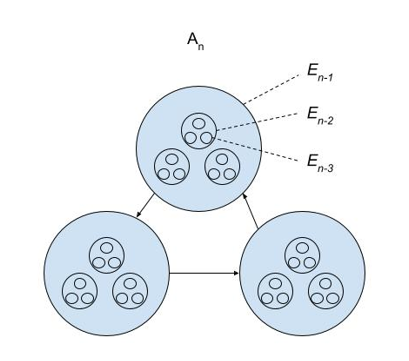
\includegraphics[scale=1]{0101DeciderX3.png}
  \caption{Decider that represents the monomial, $x^3$.}
  \label{fig:0101DeciderX3}
\end{figure}

$\\ $

$\textbf{Lemma}$. A cyclic automata is in a monomial decider.

$\textit{Proof}$. Given a deterministic automata that represents a cycle, a cyclic automata is a rational language and hence a decider can recognize the cyclic automata.

Unraveling a monomial decider can be reduced down to a cycle of 1 degree depth.

$\textbf{Theorem}$. A monimial decider can be mapped into a cycle of 1 degree depth in either direction.

$\\ $

$\textit{Proof}$. Remove the lowest level state, $S_1$ from the bottom then continue removing $S_i$ from i = 2 to n-1 until you get only the states that are at $X_n$. This is a cyclic automata.

$\\ $

Remove the top state down from the $S_{n-1}$ for each layer $S_{n-1}$ to $S_(n-n-1)$. This preserves the start and finish state for the layer $x_{n}$. This is also a cyclic automaton.

$\\ $

The next theorem states that a monomial decider has a certain form called a p-adic number. 

$\\ $

$\textbf{Theorem}$. A monomial with simple p-adic form is in a decider.

$\\ $

$\textit{Proof}$. Start with the definition of p-adic number. Show its form in general. Show that it has the same description as a monomial decider. Is this another paper?

$\\ $

\begin{figure}[H]
  \centering
  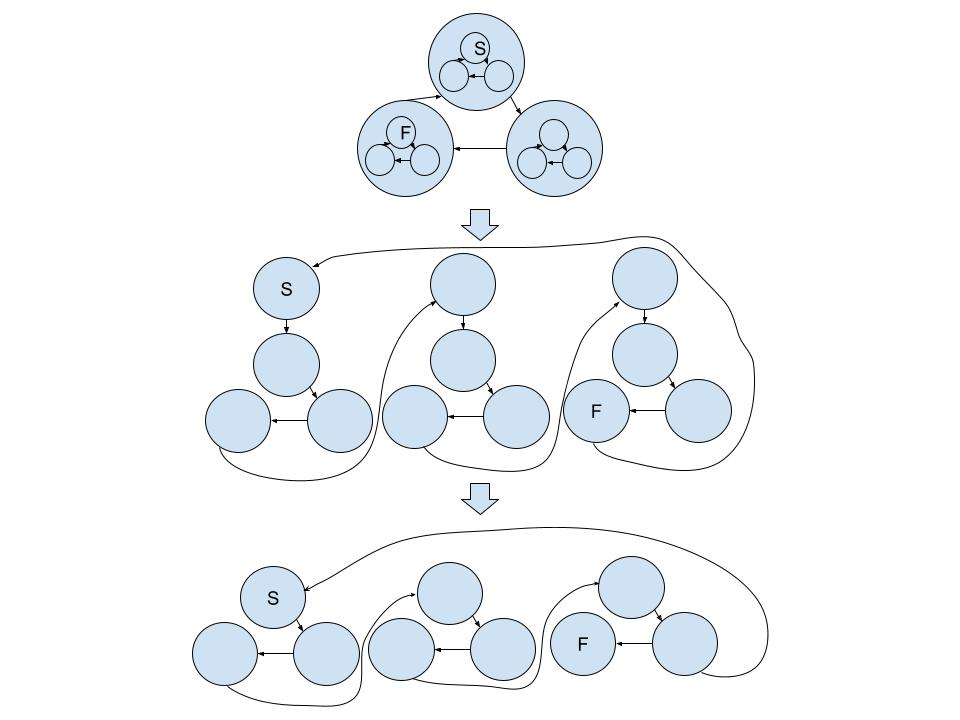
\includegraphics[width=\linewidth]{0102theorem.jpg}
  \caption{Top down removal for equivalence of decider and cyclic automata.}
  \label{fig:0102theorem}
\end{figure}

\section{Monomial of One Variable}

Given the definition of a decider:

Decider is a function $Decider<c x^n> \equiv c x^n = y$

$\\ $

A decider of at least one degree

$Decider< 3 x^4 > \equiv 3x^4 = y$

$\\ $

Contains $Decider<3 x^3> \equiv 3x^3 = y$

Contains $Decider<3 x^2> \equiv 3x^2 = y$

Contains $Decider<3 x^1> \equiv 3x^1 = y$

Contains $Decider<3 x^0> \equiv 3x^0 = y$

Hence it can be generalized to:

$Decider<c x^n>$ contains the sequence set 


$\\ $

There exists a start state and a finish state for each decider.

$\{start,...,finish\}$

$\\ $

$Decider<c x^n>,Decider<c x^{n-1}>,...,Decider<c x^0>$ 
which has a more formal definition called a rational expression. A rational expression on A over K is a semiring described as $\mathcal{E}_{n}$ such that $n\geq0$ where A is an alphabet (in our case a finite set of integers) and K is a commutative semiring. This means the following in terms of the decider

$\\ $

$Decider<c x^n>$ = $\mathcal{E}_{n}$

Contains $Decider<c x^{n-1}>$ = $\mathcal{E}_{n-1}$

...

Contains $Decider<c x^{1}>$ = $\mathcal{E}_{1}$

Contains $Decider<c x^0>$ = $\mathcal{E}_{0}$

$\\ $

The formal definition of a rational expression is defined below.

$\\ $

$\textbf{Definition. }$ $A_n = A_{n-1} \cup  {\left\{  E^* | E \in \mathcal{E}_{n-1}, (E,1)=0 \right\}}$

$\\ $

Here, $A_n$ is the set of monomials in the polynomial. $A_{n-1}$ are the monomials of degree n-1 and less of the polynomial and the set ${\left\{  E^* | E \in \mathcal{E}_{n-1}, (E,1)=0 \right\}}$ is equivalent to $Decider<cx^n>$ or equivalently the top of a single state of a decider. This theory has the opinion that it tries to describe finite recursion and nested for loops in a visual manner and, in so doing, this chain is chosen to be the best definition.

$\\ $

\begin{figure}[H]
  \centering
  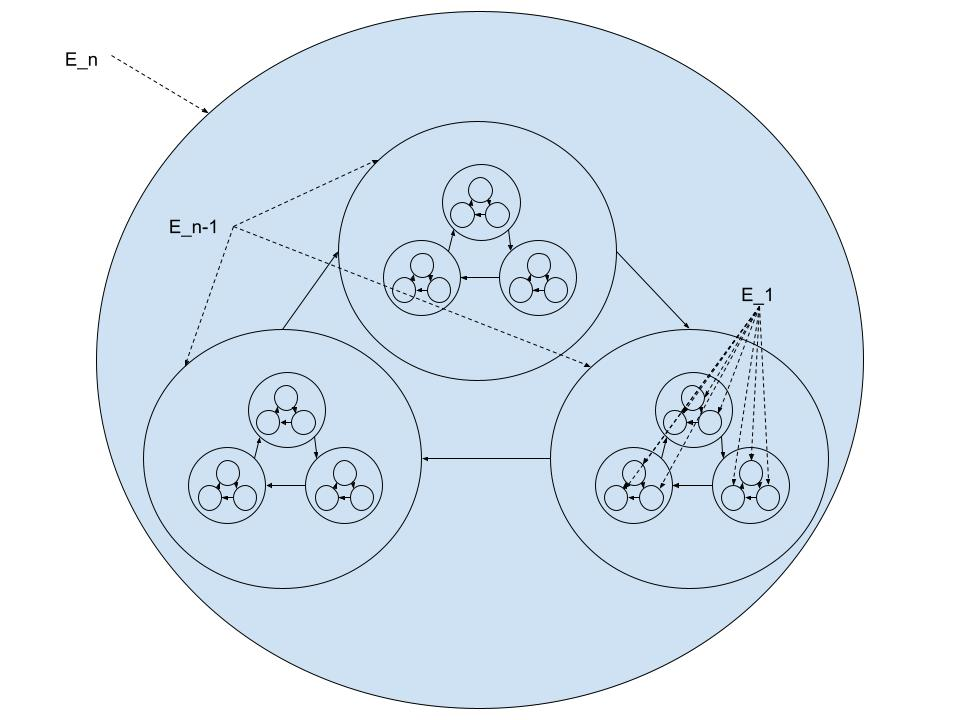
\includegraphics[width=\linewidth]{0103RationalExpression.jpg}
  \caption{Visual example of what $\mathcal{E}_n$ of a rational expression.}
  \label{fig:0103RationalExpression}
\end{figure}
Figure \ref{fig:0103RationalExpression} Visual example of $\mathcal{E}_n$ of a rational expression.

$\\ $

A rational function is defined as the following: 

$\\ $

K[x] and K[[x]]. Let K[[x]] describe a set of deciders as a polynomial representation. S is an element of K[[x]] meaning S is a decider.

$\\ $

S = $\sum_{n\geq 0}{a_n x^n}$

$\\ $


\section{Addition}

\begin{figure}[H]
  \centering
  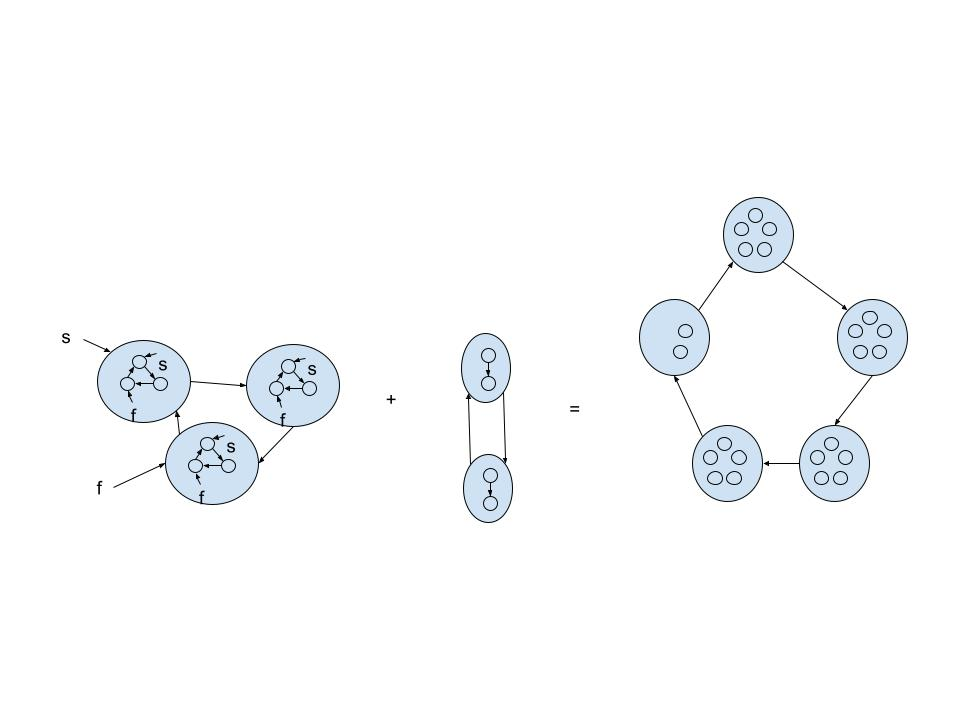
\includegraphics[width=\linewidth]{0104Addition.jpg}
  \caption{Addition of two deciders. The gradient of the circles remain the same after adding the two deciders together as the degree remains the same.}
  \label{fig:0104Addition}
\end{figure}

Given the first example:

$\\ $

$p(x)=3 x^2+4 x+5$

$p(2)=3(2)^2+4(2)+5$

$p(2)=12+8+5$

$\\ $

$m2=Decider<3 x^2>=3x^2$

$m1=Decider<4 x^1>=4 x$

$m0=Decider<5 x^0>=5$

$\\ $

Generalized to $m_x$ where x is the degree

Given polynomial functions, $p_1$ and $p_2$, they are commutative

$p_1(x)=m_a+...+m_0$

$p_2(x)=n_b+...+n_0$

$p_1(x)+p_2(x)=m_a+n_b+(m_{x+1}+n_{y+1})+...+(m_x+n_y)+...+(m_0+n_0)$ where $x=y$

$Decider<c_x x d_x>+Decider<c_y x d_y>$

$=Decider<c_x+c_y,x,d_x>=Deciders<c_x+c_y,x,d_y>$

$\implies d_x=d_y$

\section{Product}

\begin{figure}[H]
  \centering
  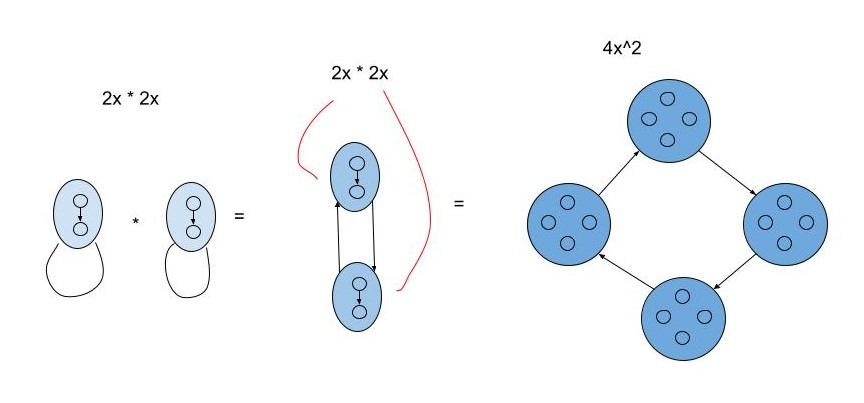
\includegraphics[width=\linewidth]{0105Product.jpg}
  \caption{Product of two deciders. The gradient of the circles get denser after adding the two deciders together as the degree increases.}
  \label{fig:0105Product}
\end{figure}

Given two monomials in the language, a and b, the product of a and b is also in the language.

$\\ $

Given $Decider<c_x x d_x>$ and $Decider<c_y x d_y>$ is in language L

Show that the product $Decider<(c_x+c_y) x d_x\times d_y>$ is in L

$Decider<c_x x d_x> \times Decider<c_y x d_y>$

$=c_x x d_x c_y x d_y$

$=c_x  x d_x+d_y$

$=(c_x+c_y) x (d_x+d_y)$ is in L

$=Decider<(c_x+c_y) x (d_x+d_y)>$

\section{Problem with Matrices}

An important problem arising from deciders is representing them as matrices. The problem can be reformulated as the following: given a polynomial p of x, show that the monomial deciders represented in the language can't be contained in a finite matrix after a set number, n, such that $x^n$.

$\\ $

$\left[ n\times n \right]\left[ n\times n \right]=\left[ m\times m \right]$ such that $m \neq n$ and $m,n\geq 0$ and $m \geq n$

$\\ $

The focus of this article pertains to the question of whether or not there exists structures with certain properties that allow law of compositions to handle the above statement. The reason why this seems feasible is because of the following proposition found in Retenaur(66).

$\\ $

$\textit{Proposition.}$ Given a proper square matrix M over $\mathcal{E}$, there exist matrices $M_1$, $M_2$ of the same size as M over $\mathcal{E}$ such that $M_1 ~1 + MM_1$ and $M_2~1+M_2M$. In particular if K is a ring, 1 - M is an invertible modulo ~.

\section{Multivariable Monomials}

\begin{figure}[H]
  \centering
  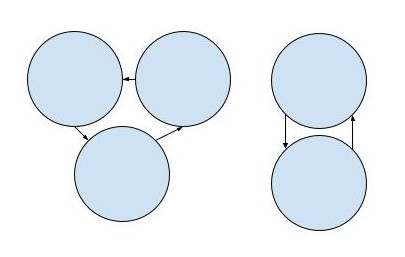
\includegraphics[scale=1]{0106Multivariables.jpg}
  \caption{Multivariable monomial deciders can be seen treated as parallel processes running next to each other.}
  \label{fig:0106Multivariable}
\end{figure}

A monomial with more than one variable can be treated the same way as handling single variables at different degrees.

$\\ $

Addition gives the following:

$\\ $

$Decider<x^6yz^3> + Decider<x^6yz^3> = Decider<2x^6yz^3>$

$\\ $

Multiplication of the decider of the same degree gives the following:

$\\ $

$Decider<cx^n> \times Decider<cy^n> \times Decider<cz^z>$

$\equiv Decider<cx^n * cy^n * cz^n>$

$\equiv Decider<cxyz^{3n}>>$

where c is some constant

$\\ $

Multiplication of the decider of the different degrees gives the following:

$\\ $

$Decider<cx^n> \times Decider<cy^m> \times Decider<cz^l>$

$\equiv Decider<cx^n * cy^m * cz^l>$

$\equiv Decider<cx^{n+m+l}>$

where c is some constant

$\\ $

Given $Decider<3xy^2>$ and $Decider<7x^7y^{-1}>$

$\\ $

$Decider<3xy^2> \times Decider<7x^7y^{-1}> = Decider<21x^8y>$

$\\ $

Representing a multivariable monomial of different degrees is a similar line of thought. There are many representations of them, however, this article will choose the simplest and have them separate as seen in figure 1.6. In this manner, multivariable monomials are a set of individual one variable monomials running simultaneously.

\section{Generalized Monomial Deciders}

\begin{figure}[H]
  \centering
  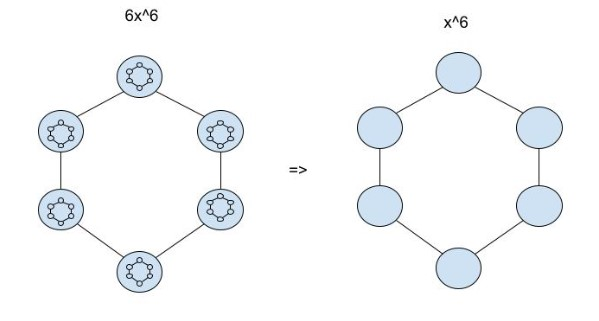
\includegraphics[scale=1]{0107Generalized.jpg}
  \caption{Generalization of a monomial decider.}
  \label{fig:0107Generalized}
\end{figure}

A decider can be represented as the top layer only if short hand notation is necessary. In a way, this removes the constant which is a term called being $\textit{proper}$, it isn't necessary true all the time. 

$\\ $

Given a Decider<m(x)> where m(x) is a monomial, keep the top layer $S_n$ in $\mathcal{E_n}$. This is called the generalized monomial decider.

\section{Concentric Monomial Deciders}

\begin{figure}[H]
  \centering
  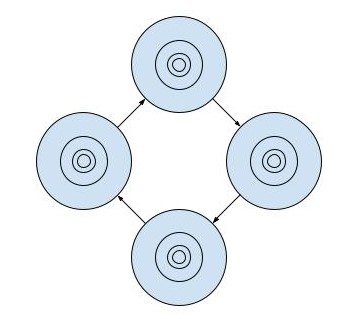
\includegraphics[scale=1]{0108Concentric.jpg}
  \caption{A concentric monomial decider is a generalized monomial decider with details missing.}
  \label{fig:0108Concentric}
\end{figure}

Generalization results in an interesting property if monomial decider is required to get in more depth. The top layer that remains from generalization remains the same and still forms a cycle, however, each state has one state and so forth up to n-1 depth.
 
\section{Constants}

\begin{figure}[H]
  \centering
  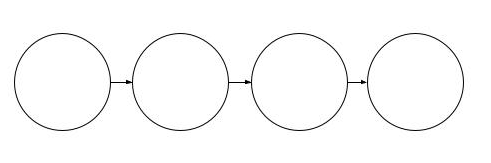
\includegraphics[scale=1]{0109Constants.png}
  \caption{A constant represented as monomial decider, $Decider<c x^0>$.}
  \label{fig:0109Constants}
\end{figure}

Given a constant, c, of a polynomial: f(x) = c, Constants are seen as linear directed acyclic graphs.

$\\ $

$Decider<c x^0> \equiv c = y$

$\\ $

Addition gives the following:

$Decider<c_1 x^0> + Decider<c_2 x^0> \equiv Decider<(c_1+c_2) x^0> \equiv Decider<c_1 + c_2>$

$\\ $

Multiplication gives the following: 

$Decider<c_1 x^0> \times Decider<c_2 x^0> \equiv Decider<c_1 c_2 x^0> \equiv Decider<c_1 c_2>$

$\\ $

There is no state in the decider where it loops back to the start. The constant is what separates a decider from a strictly mathematical cyclic object, semi-simple groups. This paper will mainly cover the cyclic part of the language.

\section{Division}

There are a finite amount of permutations, called decision functions, in a decider.

$\\ $

\begin{figure}[H]
  \centering
  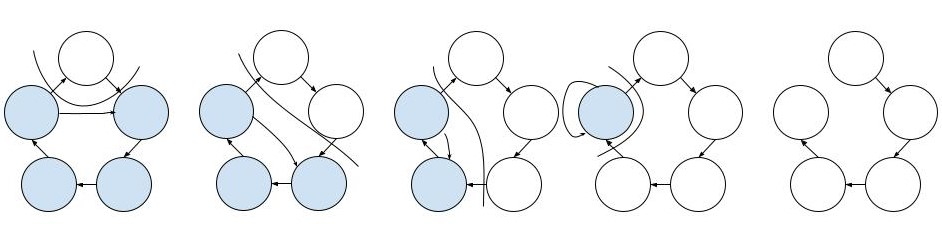
\includegraphics[width=\linewidth]{0110x5.jpg}
  \caption{One decision function of $Decider<x^5/x>$ to one decision function of $Decider<x^5/x^5>$.}
  \label{fig:0110x5overx}
\end{figure}

$\textit{Example}$. The following are deciders related to $x^5/x^i$ such that $0 \leq i \leq 5$.

$Decider<x^5 / x> \equiv Decider<x^5>/Decider<x^1>$

$Decider<x^5 / x^2> \equiv Decider<x^5>/Decider<x^2>$

$Decider<x^5 / x^3> \equiv Decider<x^5>/Decider<x^3>$

$Decider<x^5 / x^4> \equiv Decider<x^5>/Decider<x^4>$

$Decider<x^5 / x^5> \equiv Decider<x^5>/Decider<x^5>$

$\\ $

\section{Multiple Divisions}

\begin{figure}[H]
  \centering
  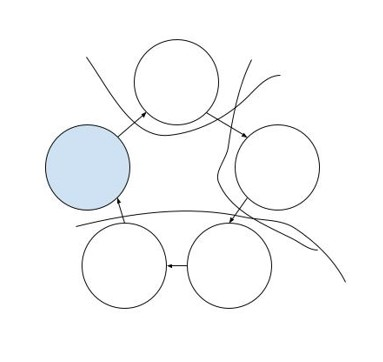
\includegraphics[width=\linewidth]{0111MultipleDivisions.jpg}
  \caption{$Decider<x^5/x/x/x^2>$}
  \label{fig:0111MultipleDivisions}
\end{figure}

$\\ $

Given multiple operations of division, this forms a topological space where the order of operations are ignored.

$\\ $

$Decider<x^5/x^2/x/x> ~ Decider<x^5/x^2/x^2>$.

$Decider<x^5/x^2/x^1/x^1> ~ Decider<x^5/x^2/x^2>$

$\\ $

The topology of the operations on the cyclic structure of a decider forms its own area of study. A topology of a decider used in this paper is constructed below.

$\\ $

$\textbf{Definition}$. A topology on a set X is a collection $\tau$ of subsets of $X$ having the following properties:

1. $\emptyset$ and $X$ are in $\tau$

2. The union of elements of any sub-collection of $\tau$ is in $\tau$

3. The intersection of the elements of any finite sub-collection of $\tau$ is in $\tau$

$\\ $
A set X for which a topology $\tau$ has been specified is called a $\textbf{topological space}$. These three properties are used as template to construct a decider.

$\\ $

A decider of a monomial can have no decision functions or a set of decision functions so $\emptyset \in \tau$ or $D \subseteq \tau$

$\\ $

The union of sets of decision functions, $D$, of $\tau$ is in $\tau$.

$\\ $

$d_1, d_2 \in D \subseteq \tau$ such that $d_1 \cup d_2 \subseteq D \subseteq \tau$ implies $d_1, d_2 \in \tau$.

$\\ $

The intersection of sets of decision functions, $D$, of $\tau$ is in $\tau$. 

Given $d_1 \in D_1$ and $d_1 \in D_2$, then $d_1 \in D_1 \cap D_2 \subseteq \tau$.

$\\ $

Using the construction above, a general categorization of the states of a decider can be illustrated to find basic patterns using a term in topology called the basis.

$\\ $

$\textbf{Definition}$. If $X$ is a set, a basis for topology on X is a collection $\textit{B}$ of subsets of $X$ such that:

1. For each $x \in X$, there is at least one basis element $B$ containing $x$

2. If $x$ belongs to the intersection of two basis elements $B_1$ and $B_2$, then there is a basis element $B_3$ containing $x$ such that $B_3 \subset B_1 \cap B_2$.

$\\ $

A decision function has a start state and two possible outcomes, accept and reject. It can be generalized that there are three kinds of states - start, accept, and reject. These form a basis - $B_{start}$, $B_{accept}$, and $B_{reject}$. Each basis element has at least one state. A state can be in the basis elements of start and accept or start and  reject meaning that the intersection forms another basis element - the intersection of two basis elements. Thus, this is the topology of a decision function generated by $B_{start}$, $B_{accept}$, and $B_{reject}$. 

The next basis that can be formed is one that describes the operations on $x^{n+k}/Q(x^k)$ where Q is the divisions (e.g. $x^6/x^3/x^2$ where $Q(x^k)=x^3/x^2$). There are $6*2+6*1=18$ permutations possible in the example given. The basis elements that form $B_{6*2}$ and $B_{6*1}$ can be described. As a programmer, this statement means that even though there are many ways to write a function, there a finite amount of different combinations to write them in terms of having be as re-factored well.
 
\section{Equivalence}

\begin{figure}[H]
  \centering
  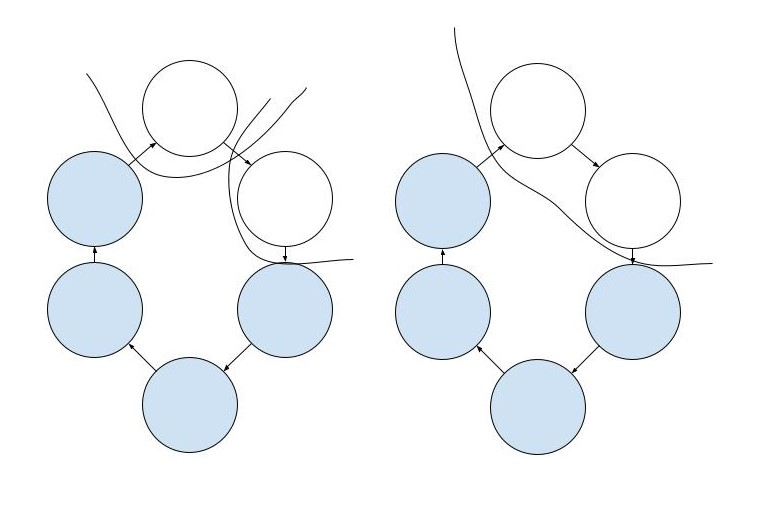
\includegraphics[width=\linewidth]{0112Equivalence.jpg}
  \caption{$Decider<x^6/x^2>$}
  \label{fig:0112Equivalence}
\end{figure}

$Decider<x^6/x^1/x^1> ~ Decider<x^6/x^2>$

$\\ $
Determining if y is in f x is easy if we are given any monomial decider in the set of the language of polynomials and their representations has the possibility to give different representations if we consider them as representations of the function f of x.

$\\ $

$Decider<x^6/x^1/x^1> \sim Decider<x^6/x^2>$ in that they decide if y is in m(x) = $x^6/Q$

$\\ $

$\textbf{Theorem of Equivalence}$. Something on lines of $Decider<x^6/x^1/x^1> = Decider<x^6/x^2>$ such that there is some x such that the monomial represented by both deciders exists where f of x = y.

$\\ $

$\textit{Proof}$. Given $Decider<a(x,y)> = Decider<x^m> Decider<y^n>$ and the definition $Decider<b(x,y)> = Decider<y^n> Decider<x^m>$, show $Decider<a(x,y)> = Decider<b(x,y)>$.

$\\ $

Start with $Decider<a(x,y)> = Decider<x^m> Decider<y^n>$

Commute the variables because each decider decides there own monomial giving, $Decider<y^n> Decider<x^m>$.

This is equivalent to $Decider<b(x,y)>$

$\\ $

Start with $Decider<b(x,y)> = Decider<y^m> Decider<x^n>$

Commute the variables because each decider decides there own monomial giving, $Decider<x^n> Decider<y^m>$.

This is equivalent to $Decider<a(x,y)>$

\section{Reversing}

$\\ $

$Decider<x^6/x^1/x^1> \equiv $sequence of permutations such that it is equal to $\sum_{i}^{n-1}{i}$

$\\ $

$Decider<x^6/x^2> \equiv $ sequence of permutations of $x_i$, $x_j$ such that it equals n-1.

$\\ $

Is shown that by the permutation of the order of operations that $Decider<x^6/x^1/x^1>$ does not have the same number of permutations as $Decider<x^6/x^2>$

$\\ $

$\textbf{Theorem of Reversing}$. Given two representations, a,b in $Decider<m(x)/Q>$ where m(x) is monomial and Q is the division operations such that m(x)/Q $\geq $ 1, a != b implies that they don't have the same quotients space.

$\\ $

$\textit{Proof}.$ Given $Decider<a(x,y)> = Decider<x^m> Decider<y^n>$ and the definition $Decider<b(x,y)> = Decider<y^n> Decider<x^m>$, show $Decider<a(x,y)> \neq Decider<b(x,y)>$.

$\\ $

Start with $Decider<a(x,y)> = Decider<x^m> Decider<y^n>$. 

Then take $Decider<x^m y^n>$. 

Commute to get $Decider<y^n x^m>$.

This is not equivalent to $Decider<y^n> Decider<x^m> = Decider<b(x,y)>$.

$\\ $

Start with $Decider<b(x,y)> = Decider<y^n> Decider<x^m>$.

Then take $Decider<y^n x^m>$

Commute to get $Decider<x^m y^n>$

This is not equivalent to $Decider<x^m> Decider<y^n> = Decider<a(x,y)>$

\begin{figure}[H]
  \centering
  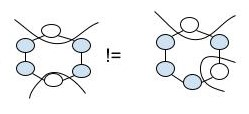
\includegraphics[scale=1]{0113Reversing.jpg}
  \caption{Two possible representations of $Decider<x^6/x/x>$.}
  \label{fig:0113Reversing}
\end{figure}

The two representations in 1.13 don't have the same quotient space and hence a != b.

\section{Corollary of Reversing}

Given a starting point of decider, the path the decider takes to decide if y is in the monomial, m(x) is unique to each representation. 

$\\ $
$\textbf{Corollary}$. Given a decider, d, in $Decider<m(x)>$ then there is path, p, that exists for d such that p = Path(d) = $s_1,s_2,...,s_i,...,s_n$ where i is count of the states in the decider of m(x).

$\\ $

$\textit{Example}$. Choose some x such that it is in path of $Decider<x^6/x^2>$ where $p = 001111$ then the following graph is what the decider is represented as.

\begin{figure}[H]
  \centering
  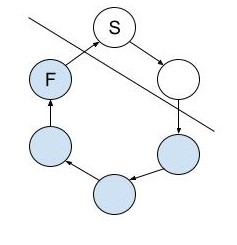
\includegraphics[scale=1]{0114CorollaryOfReversing.jpg}
  \caption{Path of one representation of $Decider<x^6/x^2>$.}
  \label{fig:0114CorollaryOfReversing}
\end{figure}

\section{Godel's Theorem}

We see that there exists two statements from these theorems

$\\ $

1. $x = x$ from a theorem of equivalence

2. $x != x$ from a theorem of reversal

$\\ $

$\textbf{Example}$: Given some $d_1$,$d_2$,$d_3$,...,infinity in decision functions in $Decider<m(x)>$

$\\ $

1. $d_1 = d_2 = d_3 = ... = infinity$

2. $d_1 != d_2 != d_3 = ... != infinity$

$\\ $


\begin{figure}[H]
  \centering
  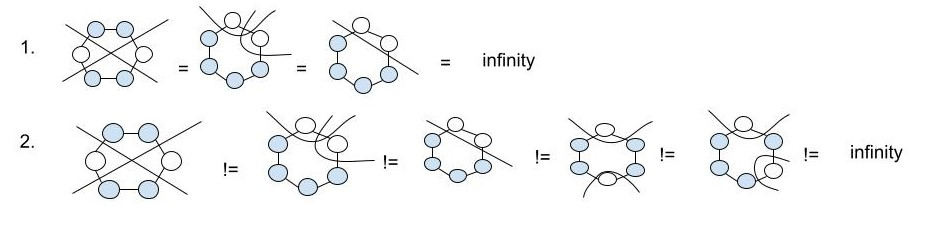
\includegraphics[width=\linewidth]{0115Godels.jpg}
  \caption{Godel's illustrated from $Decider<x^6/x^2>$.}
  \label{fig:0115Godels}
\end{figure}

$\\ $

The different representations of a monomial through the language of monomial deciders will give the problem of undecidability. This means that despite many formal definitions of the monomial decider, there is no way to solve the problem of finding a specific representation of a monomial decider without having to guess or apply some sort of probability to it. Relating to the real line, given a real line a,b a $\leq$ b, there is infinite choices between a and b. As long as b and a $\geq $ 0, there requires some sort of probability of choosing some specific number that is between a and b.

\section{Constructing The One Way Function}

A probability exists to find a certain monomial decider in the set of it's variations. A/B = Probability where A is the monomial decider we want and B is the number of all the variations.

$\\ $

$\textit{Example}$: $d_1$,$d_2$,...,$d_6$ in $Decider<x^6>$ such that $d_i$ are all distinct. 

Choose one of the deciders in D through probability

Probability of choosing d in D is 1/6 so 0.16666667

\begin{figure}[H]
  \centering
  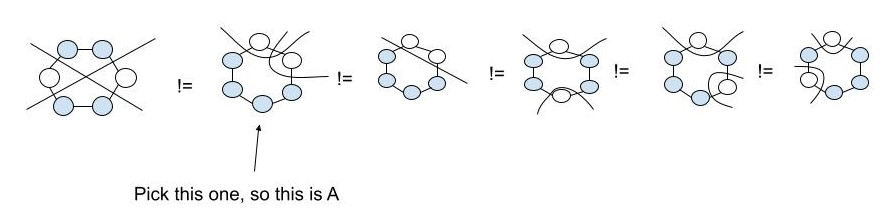
\includegraphics[width=\linewidth]{0116Constructing.jpg}
  \caption{Picking a decision function, d, from $Decider<x^6/x^2>$.}
  \label{fig:0116Constructing}
\end{figure}


$\\ $

This is called the picking function and every time it is called, the probability is multiplied such that it is $n^k$. As an example, if the picking function is called twice using the example above, it is shown that the probability is:

$1/6 \times 1/6 = 1/6^2 = 1/36 = 02777778$

$\\ $

This is formally known as the one way function.

% Chapter Template

\chapter{Analysis of Fibonacci} % Main chapter title

\label{ChapterX} % Change X to a consecutive number; for referencing this chapter elsewhere, use \ref{ChapterX}


%----------------------------------------------------------------------------------------
%	SECTION 2
%----------------------------------------------------------------------------------------

%\section{Starting With A Theorem Of Infiniteness}

%This section assumes that both P=NP and P!=NP and the following sections will %provide reasoning and examples.

%\section{Mapping Out Representations}

%This section contains my opinions of what mathematics is.

\section{Euler's Constant}

From the the reinterpretation of the theory, Euler's constant is an example of P = NP because of it's use of calculus. Euler's constant can be defined as 

$\\ $

$e = \sum_{n=0}^{\infty }\frac{1}{n!}$

$\\ $

To show that it is also in the problem set of P $\neq$ NP, start by using the picking function going into infinity. The constant $e$ is the sum of the infinite series of $\frac{1}{n!}$ and can be represented as a series of monomials representing the Decider<x> using the picking function.

$\\ $

$e = (\sum_{n=0}^{\infty }\frac{1}{n!})$

$\\ $

$e = 1 + 1 + 1/(1+1) + 1/(3+3) + 1/(4+(4*3+4*2)+4) + ...$

$\\ $

$e = p_f(Decider<x^0>) + p_f(Decider<x>)+ p_f(Decider<x^2/x> + ...$

\begin{figure}[H]
  \centering
  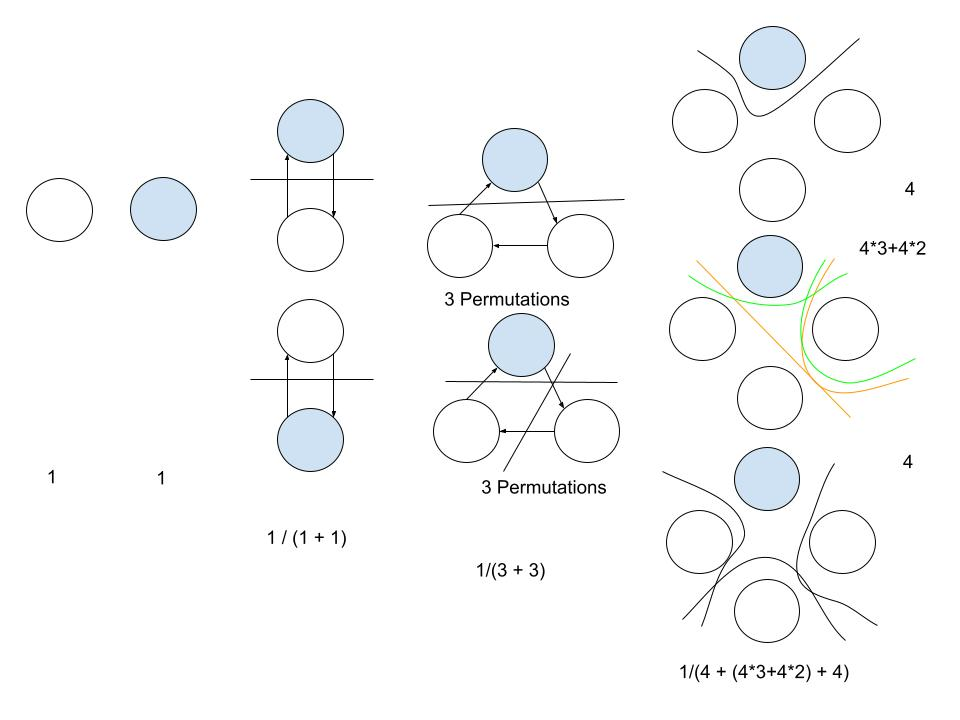
\includegraphics[scale=0.4]{0201Eulers.jpg}
  \caption{Decider that represents the first four terms of the constant $e$.}
  \label{fig:0201Eulers}
\end{figure}



\section{Example of a Decider}

The following is an example of code that roughly sketches a generalized monomial decider, Decider<$2x^2$>. It tests to see if y is in the monomial m(x) = $2x^2$. Although approximation and binary search algorithms work, using this method allows for simplicity of technique in representing a decider visually and gives the reader hands-on potential if they want to experiment on the subject further.

$\\ $

% Turn into pseudocode eventually.

\begin{lstlisting}
bool generalizedDecider(int y)
{
    if (y == 0)
    {
        return true;
    }
    var s = y;
    while (s >= 0)
    {
        for (int i = 0; i < 2; i++)
        {
            for (int j = 0; j < 4; j++)
            {
                if (s == 0 && (j == 0 || j == 2) && i == 0)
                {
                    return true;
                }
                else if (s < 0)
                {
                    return false;
                }
                s -= 1;
            }
        }
    }
    return true;
}
\end{lstlisting}

$\\ $

The above code can be represented visually as follow:

\begin{figure}[H]
  \centering
  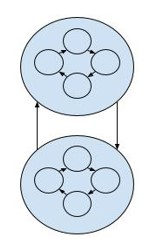
\includegraphics[scale=1]{0202Generalized.jpg}
  \caption{Decider that represents the monomial, $x^3$.}
  \label{fig:0202Generalized}
\end{figure}

\section{Analysis of the Decider $2x^2$}

Data can be extracted to find insight and build a general technique using the generalizedDecider function above for the Decider<$2x^2$>. 


$\\ $

\begin{figure}[H]
  \centering
  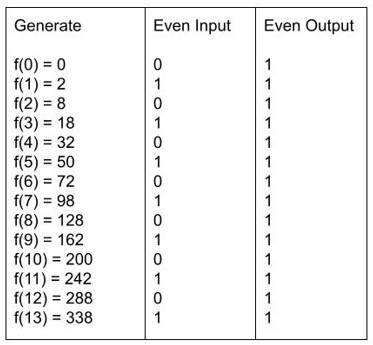
\includegraphics[scale=1]{0203Generate.jpg}
  \caption{Generate function, $2x^2$.}
  \label{fig:0203Generate}
\end{figure}

$\\ $

$\textbf{Generate}$ is f(x) = $2x^2$ = y on the first line and the number of negatives is on the second. There are two finishing and all the even parity outputs end in one state and all the odd parity outputs end on the other. $\textbf{Even Input}$ is the boolean parity of the input being even. $\textbf{Even Output}$ is the boolean parity of the output being odd. 

Here, it can be seen that there is repeating pattern of even and odd values of the following:

$\\ $

$\left[ {\begin{array}{cc}
    1 & 1 \\
    0 & 1 \\
  \end{array} } \right]$

$\\ $

From this array, two finishing states are described. When the input and output are both even and one where the input is odd and the output is even. Every time the head of the tape passes a finishing state, the count of the variable, $\textbf{visit }$is increased by one. Counting the number of visits two the finishing states, it can be seen that for every pair, (start,end), there is a difference of three for $Decider<2x^2>$. The following is a table of the results:

\begin{figure}[H]
  \centering
  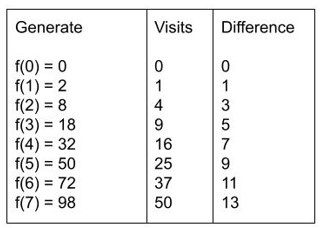
\includegraphics[scale=1]{0204Visits.jpg}
  \caption{Analysis of visits to finishing states in, $2Decider<2x^2>$.}
  \label{fig:0204Visits}
\end{figure}

From analysis, the number of times the tape head visits a finishing state is the difference of the previous input plus two. The difference increases by two every time it passes a finishing state. It doesn't pass when the number of visits is even, so it can be deduced that the difference is increased by two every time it passes the odd finishing state. This result allows us to write a program to decide if y is in $2x^2$.

$\\ $
% convert to pseudocode 

\begin{lstlisting}
bool MonomialDecider2xx(int y)
{
    var totalVisits = 0;
    var currentVisits = 0;
    var diff = 1;
    var s = 0;

    while (s <= y)
    {
        for (int i = 0; i < 2; i++)
        {
            for (int j = 0; j < 2; j++)
            {
                for (int k = 0; k < 2; k++)
                {
                    if ((i == 0) && (j == 0 || j == 1) && (k == 0))
                    {
                        if (currentVisits == totalVisits)
                        {
                            if (s == y)
                            {
                                Console.WriteLine(new String("Deciding on: " + s + " - totalVisits: " + totalVisits));
                                return true;
                            }
                            else if (s > y)
                            {
                                return false;
                            }

                            totalVisits += diff;

                            // If the tape head is on the odd finishing 
                            // state increase the diff variable by 2
                            // Do this to represent x^2 in 2x^2
                            if (i == 0 && j == 1 && k == 0)
                            {
                                diff += 2;
                            }
                        }

                        currentVisits++;
                    }
                    s++;
                }
            }
        }
    }

    return false;
}
\end{lstlisting}

\section{Representing Monomial Deciders As Code}

With the data above, the requirements on constructing a decider is as follows.

Given the function:

$\\ $

$f(x)\ =\ 2x^2 = \left\{ 0,2,8,18,\cdots \right\}$

$\\ $

The output of f(x) is of the following.

x is even at 0,8,32,72

x is odd at 2,18,50

$\\ $

There are four variables constructed:

Current passes records the number of times path traveled passes a finishing state.

Total number of times traveled on a finishing state needed to reach a valid decision.

Diff is the current number of diff to increment total hits by.

IsEven is if this resets back to even, increment Diff by two.

$\\ $

The following is code generated from our more formal representation of the solution.

\begin{lstlisting}
bool MonomialDecider2xx(int y)
{
    var totalVisits = 0;
    var currentVisits = 0;
    var diff = 1;
    var s = 0;

    while (s <= y)
    {
        // the constant 2
        for (int i = 0; i < 2; i++)
        {
            // the first pass of x in 2x^2
            for (int j = 0; j < 2; j++)
            {
                // the second pass of x in 2x^2
                for (int k = 0; k < 2; k++)
                {
                    if ((i == 0) && (j == 0 || j == 1) && (k == 0))
                    {
                        if (currentVisits == totalVisits)
                        {
                            if (s == y)
                            {
                                Console.WriteLine(new String("Deciding on: " + s + " - totalVisits: " + totalVisits));
                                return true;
                            }
                            else if (s > y)
                            {
                                return false;
                            }

                            totalVisits += diff;

                            // If the tape head is on the odd finishing
                            // state increase the diff variable by 2
                            // Do this to represent x^2 in 2x^2
                            if (i == 0 && j == 1 && k == 0)
                            {
                                diff += 2;
                            }
                        }

                        currentVisits++;
                    }
                    s++;
                }
            }
        }
    }

    return false;
}
\end{lstlisting}

$\\ $

\begin{figure}[H]
  \centering
  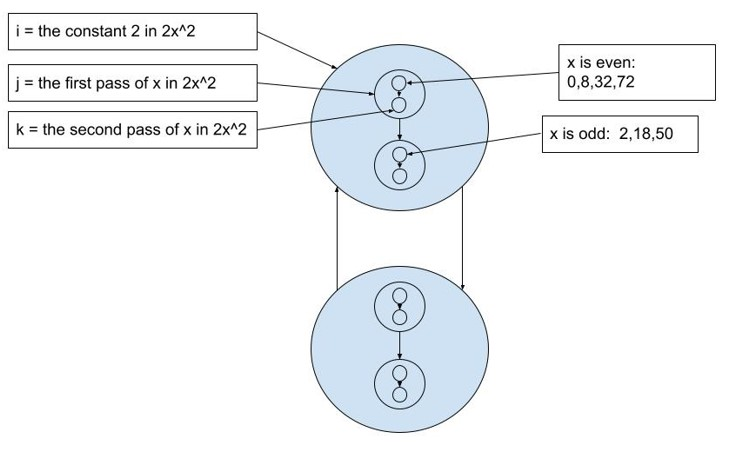
\includegraphics[width=\linewidth]{0205IdealAlgorithm.jpg}
  \caption{The algorithm described visually, $2Decider<2x^2>$.}
  \label{fig:0205IdealAlgorithm}
\end{figure}

\section{Negative Monomials}

Representing negative numbers can be thought of discretely. Below is a representation of negative numbers.

$\\ $

Addition of two negative deciders gives a negative decider.

$Decider<-x> + Decider<-x>$

$ = Decider<-x-x>$

$ = Decider<-2x>$

\begin{figure}[H]
  \centering
  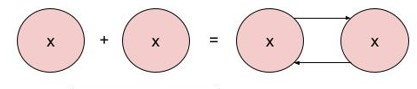
\includegraphics[scale=1]{0207Addition.jpg}
  \caption{Addition.}
  \label{fig:0207Addition}
\end{figure}

$\\ $

Cancellation of a positive and negative decider of such that it is the additive inverse, or 0.

$\\ $

$Decider<x> + Decider<-x>$

$ = Decider<x-x>$

$ = Decider<0>$

\begin{figure}[H]
  \centering
  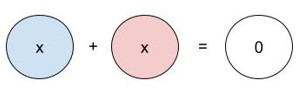
\includegraphics[scale=1]{0206Cancellation.jpg}
  \caption{Cancellation law.}
  \label{fig:0206Cancellation}
\end{figure}

$\\ $

Multiplication of two negative deciders gives a positive decider.

$\\ $

$Decider<-x> * Decider<-x>$

$ = Decider<-x*-x>$

$ = Decider<x^2>$

\begin{figure}[H]
  \centering
  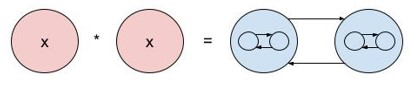
\includegraphics[scale=1]{0208Multiplication.jpg}
  \caption{Multiplication.}
  \label{fig:0208Multiplication}
\end{figure}

$\\ $

Multiplication of a negative decider with its multiplicative inverse gives a its identity, or 1.

$\\ $

$Decider<x^{-1}> * Decider<x>$

$ = Decider<x^{-1}*x>$

$ = Decider<1>$

\begin{figure}[H]
  \centering
  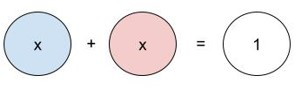
\includegraphics[scale=1]{0209MultiplicativeInverse.jpg}
  \caption{Multiplicative Inverse.}
  \label{fig:0209MultiplicativeInverse}
\end{figure}

\section{Pi}

Representing the constant pi, $\pi$, in the language of polynomials using the Leibniz formula $\pi/4 = 1 - 1/2 + 1/5 -1/7 + 1/9 + \cdots = \sum_{k=0}^{\infty} \frac{(-1)^k}{2k+1}$

$\\ $

\begin{figure}[H]
  \centering
  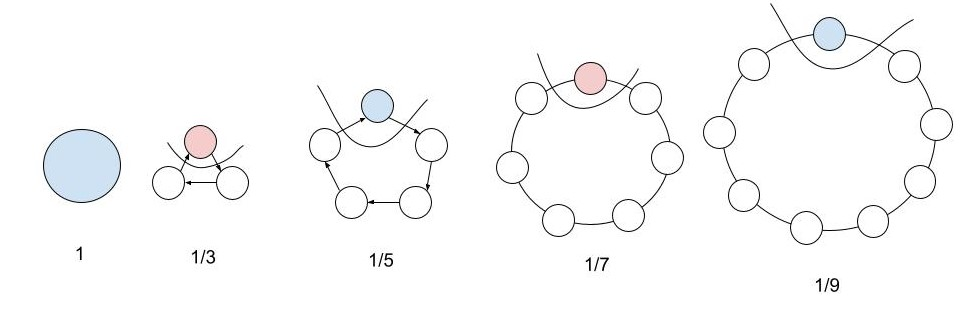
\includegraphics[width=\linewidth]{0210Pi.jpg}
  \caption{Pi under the Leibniz formula to illustrate choosing one state in a decision function of a term decider.}
  \label{fig:0210Pi}
\end{figure}

\section{Analysis of Fibonacci}

A Fibonacci sequence is a sequence of typically seen as the following, ${1,1,2,3,5,8,13,21,\cdots}$. The general formula for this sequence is:

$\\ $

$a_n = a_{n-1} + a_{n-2}$ given $a_0$ and $a_1$

$\\ $

From the example above, we see that f(1) = 1 and f(2) = 2. If we add f(1) and f(2) together we get f(3) = 3 and so on and so forth. The algorithm below will be used to collect data to be analyzed to find a general pattern:

$\\ $

\begin{lstlisting}
int fibonacci(int n)
{
    if (n == 0)
    {
        return 0;
    }

    int y = 1;
    int y1 = 1;
    int y2 = 0;

    for(int i = 1; i < n; i++)
    {
        y = y1 + y2;
        y2 = y1;
        y1 = y;
    }

    return y;
}
\end{lstlisting}

$\\ $

The data collected is organized into input, its parity, output, and its parity. First, the input and its parity value is analyzed in the following:

$\\ $

\begin{figure}[H]
  \centering
  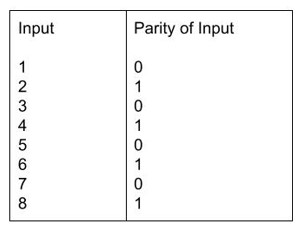
\includegraphics[scale=1]{0211Fibonacci.jpg}
  \caption{The input and the parity of the input of Fibonacci.}
  \label{fig:0211Fibonacci}
\end{figure}

The parity alternates between 0 and 1 which doesn't mean much on its own. Collecting data from the output of the sequence function gives the following:

\begin{figure}[H]
  \centering
  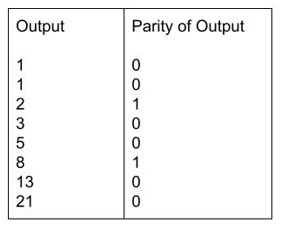
\includegraphics[scale=1]{0212Fibonacci.jpg}
  \caption{The output and the parity of the output of Fibonacci.}
  \label{fig:0212Fibonacci}
\end{figure}

On analysis, it can be seen that there are two patterns mapped out - one from input values 1, 2, and 3 (called {123}) and one from input values 4, 5, and 6 (called {456}). Laying these findings flat on a $3 \times 3$ matrix gives the following:

\begin{figure}[H]
  \centering
  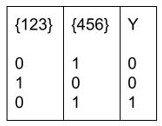
\includegraphics[scale=1]{0213Fibonacci.jpg}
  \caption{The output Y is the output parity.}
  \label{fig:0213Fibonacci}
\end{figure}

There are two matrices that form from analysis of the parity of the input and output. Using the technique to develop an algorithm for the $Decider<2x^2>$ it can be concluded that there are three finishing states for each matrix giving a total of six different finishing states.

\section{Modeling Deciders of Fibonacci}

There exists a mapping between the determinants of the Fibonacci sequence to each state of the Fibonacci sequence. On analyzing the parity of the input of {123}, {456} and the output of the fibonacci sequence, two matrices emerge. Label the input {123} as $E_1$, the input of {456} as $E_2$, and the output of the Fibonacci sequence as $E_3$.

$\\ $

$\begin{array}{ccc}
E_1 & E_2 & E_3\\
0 & 1 & 0\\
1 & 0 & 1\\
0 & 1 & 1\\
\end{array}$

$\\ $

There are six permutations pivoting by the row of the matrices. Three of them have a determinant of -1 and the other three have a determinant 1. The three matrices that have the determinant of -1 are as follows.

$\\ $

$M_1 = \begin{array}{ccc}
E_1 & E_2 & E_3\\
0 & 1 & 0\\
1 & 0 & 1\\
0 & 1 & 1\\
\end{array}$

$\\ $

$M_2 = \begin{array}{ccc}
E_1 & E_2 & E_3\\
1 & 0 & 1\\
0 & 1 & 1\\
0 & 1 & 0\\
\end{array}$

$\\ $

$M_3 = \begin{array}{ccc}
E_1 & E_2 & E_3\\
0 & 1 & 1\\
0 & 1 & 0\\
1 & 0 & 1\\
\end{array}$

$\\ $

The next three matrices that have a determinant of 1 is as follows.

$\\ $

$M_4 = \begin{array}{ccc}
E_1 & E_2 & E_3\\
0 & 1 & 0\\
0 & 1 & 1\\
1 & 0 & 1\\
\end{array}$

$\\ $

$M_5 = \begin{array}{ccc}
E_1 & E_2 & E_3\\
1 & 0 & 1\\
0 & 1 & 0\\
0 & 1 & 1\\
\end{array}$

$\\ $

$M_6 = \begin{array}{ccc}
E_1 & E_2 & E_3\\
0 & 1 & 1\\
1 & 0 & 1\\
0 & 1 & 0\\
\end{array}$

$\\ $

Let's take $M_1$ and model the Fibonacci sequence and swap the rows $E_1$ and $E_2$ to get us $N_1$. The determinant of $N_1$ is 1 and the rows still have integrity. The matrices can be turned into a sort of adjacency matrix and mapping the the entries of $E_1$ of $M_1$ and $E_2$ of $N_1$ to the value of the states can be seen as a graph in the following:

$\\ $

$E_1 \equiv -x = y - z$

Determinant of $M_1$ = -1

$\\ $

\begin{figure}[H]
  \centering
  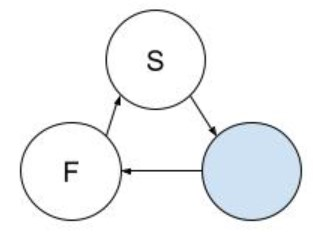
\includegraphics[scale=1]{0214E1.jpg}
  \caption{The determinant of input parity $E_1$ of $M_1$ modeled as a graph visually.}
  \label{fig:0214E1}
\end{figure}


$\\ $

$E_2 \equiv x = -y + z$

Determinant of $N_1$ = 1

$\\ $

\begin{figure}[H]
  \centering
  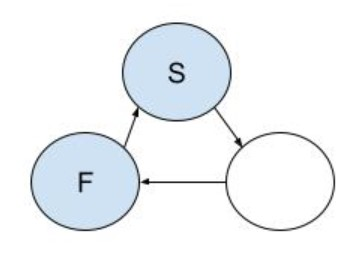
\includegraphics[scale=1]{0215E2.jpg}
  \caption{The determinant of input parity $E_2$ of $N_1$ modeled as a graph visually.}
  \label{fig:0215E2}
\end{figure}

$\\ $ 

Taking the sum of the path of the graph and mapping the state's that represent 0 to -1, the following can be seen.

$\\ $

$E_1 \equiv -x = y - z$

Path of $M_1$ = -1 + 1 - 1 = -1

$\\ $

\begin{figure}[H]
  \centering
  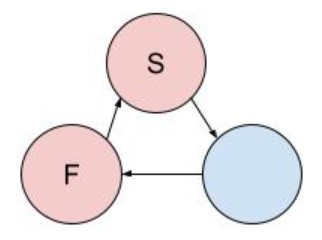
\includegraphics[scale=1]{0216E1.jpg}
  \caption{The sum of input parity $E_1$ of $M_1$ modeled as a graph visually.}
  \label{fig:0216E1}
\end{figure}


$\\ $

$E_2 \equiv x = -y + z$

Path of $N_1$ = 1 - 1 + 1 = 1

$\\ $

\begin{figure}[H]
  \centering
  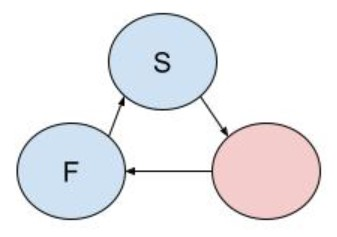
\includegraphics[scale=1]{0217E2.jpg}
  \caption{The sum of input parity $E_2$ of $N_1$ modeled as a graph visually.}
  \label{fig:0217E2}
\end{figure}

$\\ $ 

\section{Redrawing the Fibonacci Sequence}

From our analysis, it can be seen that there are three states that are a minimum to create a fibonacci sequence. Minimization gives us a monomial generator, ${S_x,S_y,S_z}$. Set the three states to a desired configuration and it will generate the fibonacci sequence. It can shown that it requires three states minimum to generate the fibonacci sequence.

$\\ $

Generator

$S_x = S_y + S_z$

$S_y = S_z + S_x$

$S_z = S_x + S_y$

Using the above, dynamic programming can be modeled as a set of generator functions.

\begin{lstlisting}
int fibonacciGenerator(int n)
{
    int stateX = 0;
    int stateY = 1;
    int stateZ = 1;
    int cycles = 0;

    while (cycles <= n)
    {
        cycles++;

        if (cycles > n)
        {
            return stateX;
        }

        stateX = stateY + stateZ;
        Console.WriteLine("stateX: " + stateX + "\tstateY: " + stateY + "\tstateZ: " + stateY);
        
        cycles++;

        if (cycles > n)
        {
            return stateY;
        }

        stateY = stateX + stateZ;
        Console.WriteLine("stateX: " + stateX + "\tstateY: " + stateY + "\tstateZ: " + stateY);

        cycles++;

        if (cycles > n)
        {
            return stateZ;
        }

        stateZ = stateX + stateY;
        Console.WriteLine("stateX: " + stateX + "\tstateY: " + stateY + "\tstateZ: " + stateY);
    }

    return stateX;
}
\end{lstlisting}

\section{The Fibonacci Decider}

Given the two monomial deciders we found using the determinant, we know that we must have six numbers in the sequence to decide if they form a Fibonacci sequence. In order to create this decider, we use an addition operator to merge them together because they cancel each other out. All deciders in each set must be true in order for the sequence to be a valid Fibonacci sequence.

\section{The Fibonacci Picking Function}

Now, let's apply the picking function, pf, to the fibonacci decider and show the probability, $P_r$, of finding a sequence. $pf({xyz}_1 + {xyz}_2) = Pr({xyz}_1)*Pr({xyz}_2) \leq 1/n^{k}$

Each decider has 3 representations giving $3^2 = 9$ total for each set. We pick one decider in each set to get the probability.

There are 6 deciders with 6 permutations giving $6^2 = 36$ permutations.

This shows a concrete example of the picking function which is a type of one way function.
 
% Chapter Template

\chapter{Inferrable Languages} % Main chapter title

\label{ChapterX} % Change X to a consecutive number; for referencing this chapter elsewhere, use \ref{ChapterX}

%----------------------------------------------------------------------------------------
%	SECTION 1
%----------------------------------------------------------------------------------------

\section{Introduction}

The concept of statistics and blackboxes has been drawn out extensively in theories and applications for decades but what of languages and knowing what word can be used to generate the next series of words? Everyone guesses what words can come out of someone talking given enough experience. In this article, the idea of inferrable languages is presented which are languages that allow the next series of words in the sequence to be inferred given enough samples in the sequence.


\section{Applying The Fibonnaci Decider}

Given the definition of the Fibonacci decider and a Lindenmayer system, insight can be derived from to that there exists the commutative and non-commutative properties of the operations. Let the Fibonacci decider for $x_1$, $y_1$, $z_1$ have a determinant equivalent to the identity, -1, then the Fibonacci decider for $x_2$, $y_2$, $z_2$ have a determinant inverse to the identity, 1. The decision functions represented on the six variables is shown below.

$\\ $

$\textbf{Decider}$ for $x_1$, $y_1$, $z_1$

$-x_1 = y_1 - z_1$

$y_1 = -x_1 - z_1$

$-z_1 = x_1 - y_1$

$\\ $

$\textbf{Decider}$ for $x_2, y_2, z_2$

$x_2 = y_2 - z_2$

$-y_2 = x_2 - z_2$

$z_2 = x_2 - y_2$

$\\ $

The Fibonacci decider is a six variable machine on $x_1$, $y_1$, $z_1$, $x_2$, $y_2$, and $z_2$ that decides if the six words are consecutive to each other so that it can completely infer the morphisms of the variables on the sequence.

$\\ $

$\textbf{Fibonacci Decider}$

$x_1 = -y_1 +z_2 - x_2 + y_2 - z_1$

$-y_1 = z_2 - x_2 + y_2 - z_1 + x_1$

$z_2 = -x_2 + y_2 - z_1 + x_1 - y_1$

$-x_2 = y_2 - z_1 + x_1 - y_1 + z2$

$y_2 = -z_1 + x_1 - y_1 + z_2 - x_2$

$-z_1 = x_1 - y_1 + z_2 - x_2 + y_2$

$\\ $

With the Fibonacci decider constructed, apply this concept with a Lindenmayer system. Lindenmayer systems are structures that were originally developed by Aristid Lindenmayer to describe how plants grow. They are simple systems that can be used to model generative concepts. Mathematically speaking, a Lindenmayer system is a deterministic, context-free grammar (shorthand name is D0L systems) defined below.

$\\ $

$\textbf{Lindenmayer System}$

L is the definition of the D0L System

$L = (V,\omega,P)$

$V$ are the characters in the language called the alphabet

$\omega$ is the starting string called the start

$P$ are the production rules in the language called the rules
$\\ $


$\\ $
$\textit{Example 3.2.1}$. As an example the Fibonacci sequence is defined as the sequence below.

$\textit{alphabet}$. $= \{a,b\}$

$\textit{rules}$. $= \{a \Rightarrow ab, b \Rightarrow a\}$

$\textit{start}$. $= b$

$\\ $

With the Fibonacci sequence defined as a Lindenmayer system, the rest of the chapter explains the relation with deciding if a sequence is a Fibonacci sequence and its decomposition to form a language that decides if it is inferrability.

\section{Fibonacci DOL Decider Left Hand Side}

Representing the left hand side of the Fibonacci sequence as a D0L system alphabet requires a alphabet, rules, and a starting state. The left hand side are the two deciders that are composed to form the decider on $x_1 y_1 z_1$ and $x_2 y_2 z_2$. The first six sequences of that form Fibonacci sequence is shown below.

$\\ $

$\textit{Example 3.3.1}$.

$a\ b\ ab\ bab\ abbab\ bababbab$

$\\ $

An important function with sequences and, in particular, words is the length function. Algorithms and functions that operate on words either programmatically or mathematically rely on taking their length. The following example takes the $\textit{example 3.3.1}$ and lists their length.

$\\ $
$\textit{Example 3.3.2}$.

$1\ 1\ 2\ 3\ 5\ 8\ 13\ 21$

$\\ $

A general relationship is found using the value of the length with the Fibonacci sequence and even more generally, is the concept called dynamic programming. The relationship for the sequence specifically is defined as the equation below.

$\\ $
$\textit{Example 3.3.3}$.

$T_n = T_{n-1} + T_{n-2}$

$\\ $

Here, $T_n$ is the current index of the sequence and $T_{n-1}$ and $T_{n-2}$. In the previous chapter, generators are constructed with three variables and on a more general term, it is called the recurrence relation. The Fibonacci decider is not operating on the length specifically but the entirety of its detail which means it operates on the characters of the words in the sequences which will be described in more detail later on. 

$\\ $

$\textit{Example 3.3.4}$. An example of the Fibonacci decider on variables $x_1$, $y_1$, and $z_1$.

$\textbf{Decider}$ for $x_1, y_1, z_1$

$-x_1 = y_1 - z_1$

$-y_1 = -z_1 + x_1$

$z_1 = x_1 + y_1$

$\\ $

$\textit{Example 3.3.5}$. An example of the Fibonacci decider on variables $x_2$, $y_2$, and $z_2$.

$\textbf{Decider}$ for $x_2, y_2, z_2$

$x_2 = y_2 + z_2$

$-y_2 = z_2 - x_2$

$-z_2 = - x_2 + y_2$

$\\ $

In this next example the variables with values from the Fibonacci D0L system is the set such that the conjugation is seen. A conjugation is one such that given a cyclic language and u,v such that they are words in the language, uv and vu are in the language. An example of this is seen where moving the relation of the head variable from third sequence, $z_1$, to the six sequence, $x_2$, below.

$\\ $

$\textit{Example 3.3.6}$. Setting the variables with values from the Fibonacci D0L system.

$x_1 = a$

$y_1 = b$

$z_1 = ab$

$y_2 = bab$

$z_2 = abbab$

$x_2 = bababbab$

$\\ $

$\textit{Example 3.3.7}$. Setting the variables of the decider with values in them and their corresponding column vectors. Here, the negative operation is the inverse operation such that given x,y in the alphabet, $-xy = (xy)^{-1} = y^{-1}x^{-1}$. 

$\\ $

$\textbf{Decider}$ for $x_1, y_1, z_1$

$\\ $

$\textit{\textbf{-x\textsubscript{1} = y\textsubscript{1} - z\textsubscript{1}}}$

$\textit{\textbf{-a = b - ab}}$

$-a + ab = b$

$-b - a = -ab$

$\\ $

$\textbf{-y\textsubscript{1} = -z\textsubscript{1} - x\textsubscript{1}}$

$\textbf{-b = -ab + a}$

ab - b = a

-b -a = -ab

$\\ $

$\textbf{z\textsubscript{1} = x\textsubscript{1}  + y\textsubscript{1}}$

$\textbf{ab = a + b}$

-a + ab = b

ab - b = a

$\\ $

$\textbf{Decider}$ for $x_2, y_2, z_2$

$\\ $

$\textbf{x\textsubscript{2} = y\textsubscript{2} + z\textsubscript{2}}$

$bababbab = bab + abbab$

$bababbab - abbab = bab$

$-bab + bababbab = abbab$

$\\ $

$\textbf{-y\textsubscript{2} = z\textsubscript{2} - x\textsubscript{2}}$

-bab = abbab - bababbab

-abbab - bab = -bababbab

-bab + bababbab = abbab

$\\ $

$\textbf{-z\textsubscript{2} = -x\textsubscript{2} + y\textsubscript{2}}$

-abbab = -bababbab + bab

bababbab - abbab = bab

-abbab - bab = -bababbab

$\\ $

In the next example, generalized equations are elaborated to show the relationship between the each semi-group in the Fibonacci sequence.

$\\ $

$\textit{Example 3.3.8}$. Generalized equations for $x_1$, $y_1$, and $z_1$ as it morphs to general variables $a$, $b$, and $c$, respectively.

$\\ $

$\textit{\textbf{-a = b - c}}$

$-a + c = b$

$-b - a = -c$

$\\ $

$\textbf{-b = -c + a}$

c - b = a

-b - a = -c

$\\ $

$\textbf{c = a + b}$

-a + c = b

c - b = a

$\\ $

$\textit{Example 3.3.9}$. Generalized equations for $x_2$, $y_2$, $z_2$ as it maps to $a$, $b$, and $c$, respectively.

$\\ $

$\textbf{-b = c - a}$

-c - b = -a

-b + a = c

$\\ $

$\textbf{-c = -a + b}$

a - c = b

-c - b = -a

$\\ $

$\textit{\textbf{a = b + c}}$

$a - c = b$

$-b + a = c$

$\\ $

It can be noted that each semi-group, $x_1 y_1 z_1$ and $y_2 z_2 x_2$, revolves clockwise independently from each other.

\section{Fibonacci DOL Decider Right Hand Side}

The Fibonacci decider are six consecutive word equations such that it forms the basis that decides they are able to be reduced to find the rules, or morphisms, of the Fibonacci sequence. The following word equations place one variable on the right hand side and leave the left hand side to form a matrix of strings.

$\\ $

$\textit{Example 3.4.1}$. $\textbf{Fibonacci Decider}$.

$\\ $

$x_1 = -y_1 + z_2 - x_2 + y_2 - z_1$

$-y_1 = z_2 - x_2 + y_2 - z_1 + x_1$

$z_2 = -x_2 + y_2 - z_1 + x_1 - y_1$

$-x_2 = y_2 - z_1 + x_1 - y_1 + z_2$

$y_2 = -z_1 + x_1 - y_1 + z_2 - x_2$

$-z_1 = x_1 - y_1 + z_2 - x_2 + y_2$

$\\ $

The following six word equations are taken using the six equations from above and form semi-groups where one variable is accounted on the left hand side as in Matiyasevich.

$\\ $

$\textit{Example 3.4.2}$. A decision function for $x_1$.

$\\ $

$\textbf{a = -b + abbab - bababbab + bab - ab}$

$a + ab - bab + bababbab - abbab = -b$

$b + a + ab - bab + bababbab = -abaab$

$-abbab b + a + ab - bab = - bababbab$

$bababbab - abbab + b + a + ab = bab$

$-bab + abbab - b + a = -ab$

$\\ $

$\textit{Example 3.4.3}$. A decision function for $-y_1$.

$\\ $

$\textbf{-b = abbab - bababbab + bab - ab + a}$

$-b - a + ab - bab + bababbab = abbab$

$-abbab -b-a + ab - bab = -bababbab$

$bababbab -abbab -b - a + ab = bab$

$-bab + bababbab -abbab -b -a = -ab$

$-a + ab -bab + bababbab -abbab -b  = a$

$\\ $

$\textit{Example 3.4.4}$. A decision function for $z_2$.

$\\ $

$\textbf{abbab = -bababbab + bab - ab + a -b}$

$abbab + b - a + ab - bab = -bababbab$

$bababbab + abbab + b - a + ab = bab$

$-bab + bababbab + abbab +b - a = -ab$

$ab -bab + bababbab + abbab + b = a$

$-b + a + ab + bab - bababbab + abbab = -b$

$\\ $

$\textit{Example 3.4.5}$. A decision function for $-x_2$.

$\\ $

$\textbf{-bababbab = bab - ab + a - b + abbab}$

$-bababbab - abbab + b - a + ab = bab$

$-bab -bababbab - abbab + b - a = -ab$

$ab -bab -bababbab - abbab + b = a$

$-bab + ab -a -bababbab - abbab = -b$

$- abbab + b -a ab -bab -bababbab = abbab$

$\\ $

$\textit{Example 3.4.6}$. A decision function for $y_2$.

$\\ $

$\textbf{bab = -ab + a -b + abbab - bababbab}$

$bab + bababbab - abbab + b - a = -ab$

$ab + bab + bababbab - abbab + b = a$

$-a ab + bab + bababbab - abbab = -b$

$b -a + ab + bab + bababbab = abbab$

$-abbab + b -a + ab + bab = -bababbab$

$\\ $

$\textit{Example 3.4.7}$. A decision function for $-z_1$.

$\\ $

$\textbf{-ab = a - b + abbab - bababbab + bab}$

$-ab - bab + bababbab - abbab + b = a$

$-a -ab -bab + bababbab - abbab = -b$

$b -a -ab -bab + bababbab = abbab$

$-abbab + b -a -ab -bab = -bababbab$

$-bab + bababbab -abbab + b -a -ab = bab$

\section{The Law of Commutativity and Noncommutativity}

The law of commutativity and the law of noncommutativity combined gives the law of commutativity and noncommutativity

$\\ $
 
The Law of Commutativity

a + b = b + a

ex. 8 + 5 = 5 + 8

$\\ $

The Law of Noncommutativity

a+ b != b + a

ex. 8 - 5 != 5 - 8

$\\ $

Each equation in the example on the left has permutations.

From this example, it can be implied that for every variable, n, in an equation there is $n^2$ permutations in the sequence.

The first equation is bold and italicized in the set to make a decider.



$
\begin{matrix}
 \textit{\textbf{a = b + c}} & \textbf{b = a - c} & \textbf{-c = a - b}\\
 b = a - c & b - a = -c & -c + b = a\\
 -c = a - b & b + c = a & -c - a = -b
\end{matrix}
$

\section{Operations}

Operations for the right hand side (RHS) versus the left hand side (LHS) represents different operations of the string in different scenarios.

$\\ $

RHS Evaluation

Right to Left

+ Remove from the back

- Add to the front

abaababa = - abaab + b - ab + a -aba

abaababa = - abaab + b - ab -ab

abaababa = - abaab + b - abab

abaababa = - abaab - aba

abaababa = - abaababa

$\\ $

LHS Evaluation

Left to Right

+ Remove at the front

- Add to the back

abaababa + abaab - b + ab - a = -aba

aba - b + ab - a = -aba

abab + ab - a = -aba

ab - a = -aba

aba = -aba

$\\ $

$\textit{Proposition.}$The characteristic series of a rational cyclic language is a Z-linear combination of characters of finite deterministic automata.

$\\ $

\section{Definition Of Support}

A support is defined as the following:

A* is a word

S is the function

Image by S of a word w is denoted by (S,w) and is the coefficient of w in S

Support(S) = {w in A* such that (S,w) != 0}

$\\ $

Now we take deciders of a monomial and the picking function to redefine the support of a noncommutative rational language

R is the rational numbers where x in R = a/b

such that a,b is in integers and b $\neq$ 0

Q is the quotient space represented in topology such that A/~ where are sets and ~ is the divisions of A

R-rational is the representation of R as the polynomial function

Q-rational is the representation of Q as a polynomial

\section{Rationals Of Picking Function}

Support of the Fibonacci Picking Function of the deciders of a monomial.

Q-rational-deciders are the possible monomial deciders of Q-rational-string. Use the picking function, PF, to choose one decision function in Q-rational-deciders, we see a mapping from Q-rational => R-rational.

\begin{figure}[H]
  \centering
  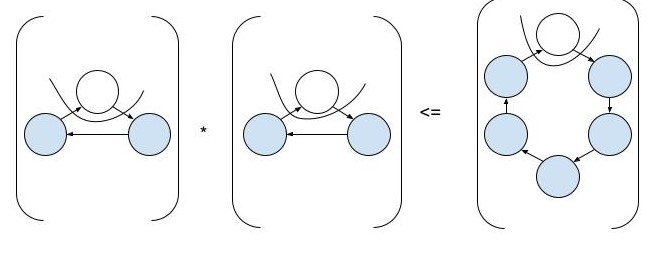
\includegraphics[width=\linewidth]{0219Rationals.jpg}
  \caption{Q rational image of the q rational string, $x^3/3$, $x^3/3$, and $X^6/x$.}
  \label{fig:0219Rationals}
\end{figure}

Deciders for $x^3/x$ has 9 possible configurations, or, in algebraic terms, permutations, and $x^6/x$ has 36 possible configurations. This equates to R rational for $x^3/x$ being $1/9$ and $x^6/x$ being $1/36$.

This implies the existence of the map between Q rational to R rational.

\section{Support Of Picking Function}

The support of an inferrable language is now defined to be:

$\\ $

Dupport of PF of Q-rational-deciders = support(PF(Q-rational-deciders))

$\\ $

Decider in Q-rational-deciders such that decider is unique $\equiv$ Determinant of a configuration of a decider != 0

\section{Law Of Strings}

$
\begin{matrix}
 \textit{\textbf{a = b + c}} & \textbf{b = a - c} & \textbf{-c = a - b}\\
 b = a - c & b - a = -c & -c + b = a\\
 -c = a - b & b + c = a & -c - a = -b
\end{matrix}
$

$\\ $

$
\begin{matrix}
 (\textit{\textbf{LHS}} = RHS) \neq (\textit{\textbf{RHS}} & \textbf{LHS})\\
 (\textit{\textbf{LHS}} = \textbf{RHS}) = (\textit{\textbf{RHS}} & \textit{LHS})\\
\end{matrix}
$

$\\ $

Condense the above to get a generalization.

$\\ $

$
\begin{matrix}
a = -a & -a = a\\
a \neq -a & -a \neq a
\end{matrix}
$

$\\ $

This is operating on variables, strings, and representations of it.

\section{Commutativity Of Addition}

$
\begin{matrix}
a + b = b - a & b - a = a + b\\
b + a = -a + b & - a + b = b + a\\
\\
a + b \neq b - a & -a + b \neq b + a\\
b + a \neq -a + b & b - a \neq a + b
\end{matrix}
$

$\\ $

Take the length function, length(s) $\equiv$ l(s), and apply to the '=' addition operations and see it's equivalence. Set b to a and reversal is accomplished.

$\\ $

$
\begin{matrix}
len(a) + len(b) = len(b)+ len(-a) \equiv 11 = 11 & len(b) + len(-a) = len(a) + len(b) \equiv 11 = 11\\
len(b) + len(a) = len(-a) + len(b) \equiv 11 = 11 & len(-a) + len(b) = len(b) + len(a) \equiv 11 = 11\\
\\
a + b \neq b - a \equiv 11 \neq 10 & -a + b \neq b + a \equiv 01 \neq 11\\
b + a \neq -a + b \equiv 11 \neq 01 & b - a \neq a + b \equiv 10 \neq 11
\end{matrix}
$

\section{Commutativity Of Multiplication}

$
\begin{matrix}
a * b = b * -a & b * -a = a * b\\
b * a = -a * b & - a * b = b * a\\
\\
a * b \neq b * -a & -a * b \neq b * a\\
b * a \neq -a * b & b * -a \neq a * b
\end{matrix}
$

\section{Additive Identity}

$
\begin{matrix}
a = -a\ for\ any\ a\ is\ equal\ to\ -a & -a\ =\ a\ where\ a\ and\ -a\ is\ 1\\
a \neq -a\ where\ a\ is\ 1\ and\ -a\ is\ 0 & -a \neq a\ where\ a\ is\ 1\ and\ -a\ is\ 0
\end{matrix}
$

The LHS and RHS are equations that test whether or not they are true or false, or in terms of computational complexity theory, it is satisfiable.
10 = 10 evaluates to true or 1.
01 != 10 evaluates to true or 1 too.

\section{Multiplicative Identity}

$
\begin{matrix}
a = -a\ where\ a\ and\ -a\ are\ 1 \equiv\ a\ represented\ as\ monomial\ decider\ loops\ once\\
a \neq -a\ where\ a\ is\ 1\ and\ -a\ is\ 0 \equiv a\ represented\ as\ a\ monomial\ decider\ loops\ once
\end{matrix}
$

\section{Additive Inverse}

The Additive Inverse

$\\ $

General Equivalence

$
\begin{matrix}
a + l = -a + r \equiv 10 = 10 & -a + r = a + l \equiv 10 = 10\\
l + a = r - a \equiv 10 = 10 & r - a = l + a \equiv 10 = 10\\
\end{matrix}
$

$\\ $

Commutativity under Equivalence

$
\begin{matrix}
a + l = r - a \equiv 10 = 10 & -a + r = l + a \equiv 10 = 10\\
l + a = -a + r \equiv 10 = 10 & r - a = a + l \equiv 10 = 10\\
\end{matrix}
$


$\\ $

General Reversal

$
\begin{matrix}
a + l \neq -a + r \equiv 10 = 01 & -a + r \neq a +l \equiv 01 = 10\\
l + a \neq r - a \equiv 10 = 01 & r - a \neq l + a \equiv 01 = 10\\
\end{matrix}
$

$\\ $

Commutativity under reversal

$
\begin{matrix}
a + l \neq r - a \equiv 10 = 01 & -a + r \neq l + a \equiv 01 = 10\\
l + a \neq - a + r \equiv 10 = 01 & r - a \neq a + l \equiv 01 = 10\\
\end{matrix}
$

$\\ $

\begin{figure}[H]
  \centering
  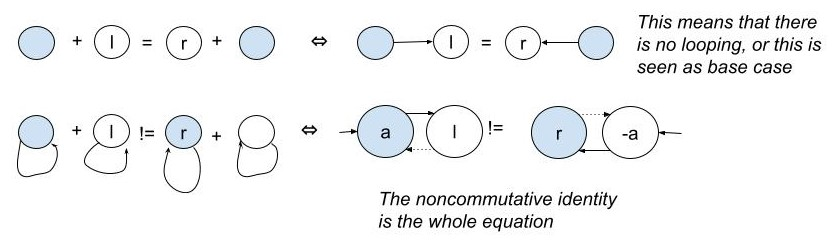
\includegraphics[width=\linewidth]{0220AdditiveInverse.jpg}
  \caption{Additive inverse direction.}
  \label{fig:0220AdditiveInverse}
\end{figure}


\section{Multiplicative Inverse}

Given a monomial such that it represents a monomial in a polynomial, if we loop around once, we see the identity path.

$\\ $

General Equivalence

$
\begin{matrix}
a * L = -a * R \equiv 10 = 10 & -a * R = a + L \equiv 10 = 10\\
L * a = R * - a \equiv 10 = 10 & R * -a = L*a \equiv 10 = 10\\
\end{matrix}
$

$\\ $

Commutativity under Equivalence

$
\begin{matrix}
a * L = R * -a \equiv 10 = 10 & -a * R = L * a \equiv 10 = 10\\
L * a = -a * R \equiv 10 = 10 & R * -a = a * L \equiv 10 = 10\\
\end{matrix}
$


$\\ $

General Reversal

$
\begin{matrix}
a*L \neq -a*R \equiv 10 = 01 & -a*R \neq a*L \equiv 01 = 10\\
L*a \neq R*-a \equiv 10 = 01 & R*-a \neq L*a \equiv 01 = 10\\
\end{matrix}
$

$\\ $

Commutative under Reversal

$
\begin{matrix}
a*L \neq R*-a \equiv 10 = 01 & -a*R\neq L*a \equiv 01 = 10\\
L*a \neq - a*R \equiv 10 = 01 & R*-a \neq a*L \equiv 01 = 10\\
\end{matrix}
$

$\\ $

\begin{figure}[H]
  \centering
  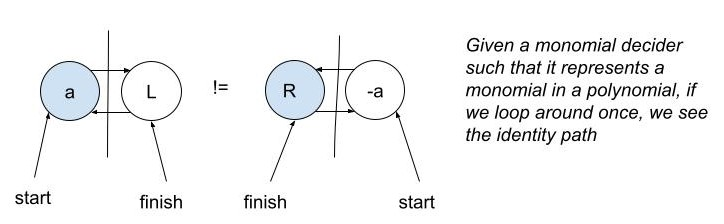
\includegraphics[width=\linewidth]{0221MultiplicativeInverse.jpg}
  \caption{Multiplicative inverse direction.}
  \label{fig:0221MultiplicativeInverse}
\end{figure}

\section{Generalized Operations}

The set of images that describes the operations on monomials can be put together to find a 2x2 matrix that describes them using the laws provided.


\begin{figure}[H]
  \centering
  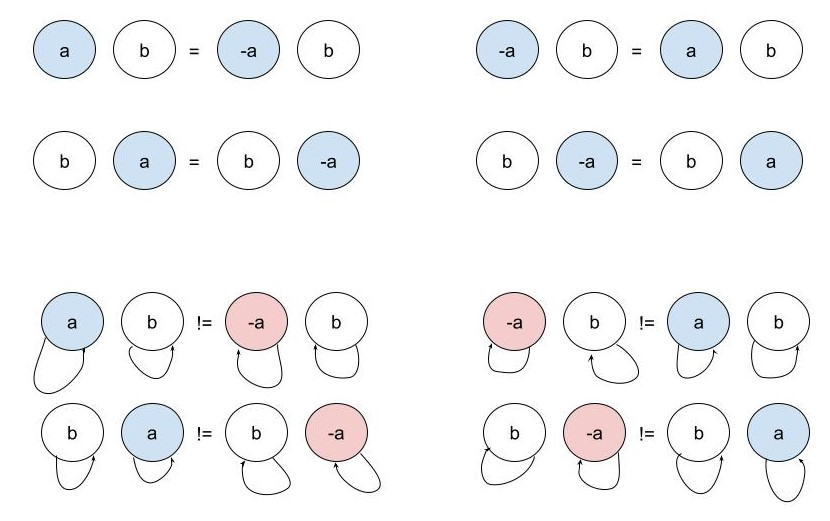
\includegraphics[width=\linewidth]{0222Operations.jpg}
  \caption{Generalized operations.}
  \label{fig:0222Operations}
\end{figure}

\section{Generalized Communativity}

For showing commutativity, have the following images to represent addition and multiplication. Fibonacci sequences are seen to be non-commutative if they are seen in this regards.

\begin{figure}[H]
  \centering
  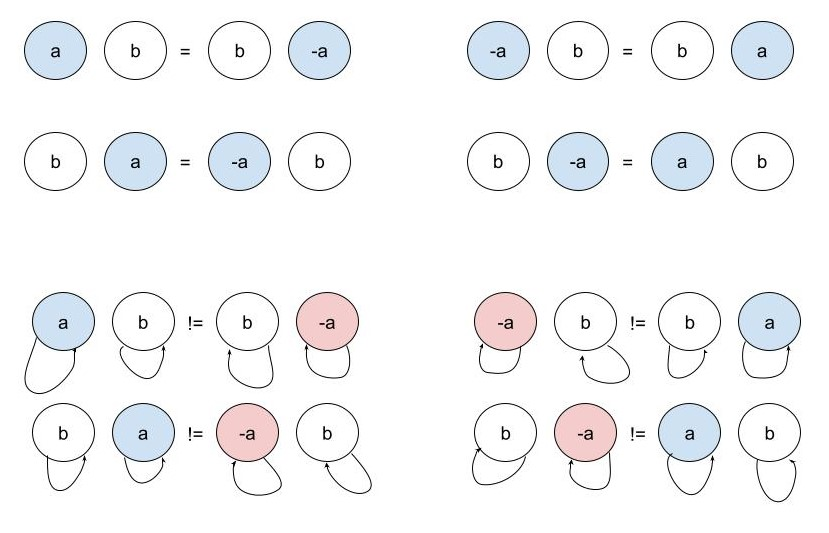
\includegraphics[width=\linewidth]{0223Commutativity.jpg}
  \caption{Communativity.}
  \label{fig:0223Commutativity}
\end{figure}

\section{Associativity Of Addition}

Associativity of addition is defined as:

a + (b + c) = (a + b) + c

\begin{figure}[H]
  \centering
  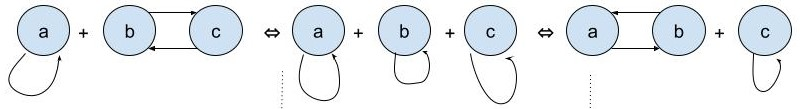
\includegraphics[width=\linewidth]{0224AssociativityOfAddition.jpg}
  \caption{Associativity of addition.}
  \label{fig:0224AssociativityOfAddition}
\end{figure}

$\\ $

a + bc

$\\ $

$
\begin{matrix}
a = -a & -a = a \\
a \neq -a & -a \neq a\\
\end{matrix}
$

$\\ $

$
\begin{matrix}
b + c = -b + c & -b + c = b + c\\
c + b\neq -c+b & -c+b \neq c + b\\\
\\
c + b= c+b & -b + c = c + b\\
c + b\neq -c+b & -c+b \neq c + b\\
\\
b + c = c-b & c-b = b + c\\
b + c\neq c-b & c-b \neq b+ c\\
\\
c + b = b + c & -c+b = b + c\\
c + b \neq b-c & -c+b \neq b + c\\
\end{matrix}
$

$\\ $

a + b + c

$\\ $

$
\begin{matrix}
a = -a & -a = a \\
a \neq -a & -a \neq a\\
\end{matrix}
$

$\\ $

$
\begin{matrix}
b = -b & -b = b \\
b \neq -b & -b \neq b\\
\end{matrix}
$

$\\ $

$
\begin{matrix}
c = -c & -c = c \\
c \neq -c & -c \neq c\\
\end{matrix}
$

$\\ $

ab + c

$\\ $

$
\begin{matrix}
a + b = -a + b & -a + b = a + b\\
b + a\neq -b+a & -b+a \neq b + a\\\
\\
b + a= b+a & -a + b = b + a\\
b + a\neq -b+a & -b+a \neq b + a\\
\\
a + b = b-a & b-a = a + b\\
a + b\neq b-a & b-a \neq a+ b\\
\\
b + a = a + b & -b+a = a + b\\
b + a \neq a-b & -b+a \neq a + b\\
\end{matrix}
$

$\\ $

$
\begin{matrix}
c = -c & -c = c \\
c \neq -c & -c \neq c\\
\end{matrix}
$


\section{Associativity Of Multiplication}

Associativity of multiplication is defined as:

a * (b*c) = (a*b)*c

$\\ $

\begin{figure}[H]
  \centering
  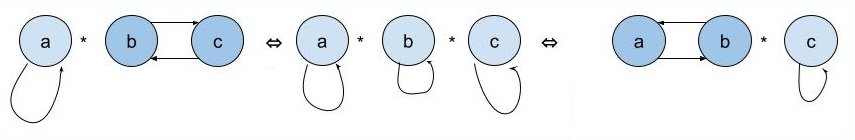
\includegraphics[width=\linewidth]{0225AssociativityOfMultiplication.jpg}
  \caption{Associativity of multiplication.}
  \label{fig:0225AssociativityOfMultiplication}
\end{figure}

$\\ $

a + bc

$\\ $

$
\begin{matrix}
a = -a & -a = a \\
a \neq -a & -a \neq a\\
\end{matrix}
$

$\\ $

$
\begin{matrix}
b * c = -b * c & -b * c = b * c\\
c * b\neq -c*b & -c*b \neq c * b\\\
\\
c * b= c*b & -b * c = c * b\\
c * b\neq -c*b & -c*b \neq c * b\\
\\
b * c = c-b & c-b = b * c\\
b * c\neq c-b & c-b \neq b* c\\
\\
c * b = b * c & -c*b = b * c\\
c * b \neq b-c & -c*b \neq b * c\\
\end{matrix}
$

$\\ $

a + b + c

$\\ $

$
\begin{matrix}
a = -a & -a = a \\
a \neq -a & -a \neq a\\
\end{matrix}
$

$\\ $

$
\begin{matrix}
b = -b & -b = b \\
b \neq -b & -b \neq b\\
\end{matrix}
$

$\\ $

$
\begin{matrix}
c = -c & -c = c \\
c \neq -c & -c \neq c\\
\end{matrix}
$

$\\ $

ab + c

$\\ $

$
\begin{matrix}
a * b = -a * b & -a * b = a * b\\
b * a\neq -b*a & -b*a \neq b * a\\\
\\
b * a= b*a & -a * b = b * a\\
b * a\neq -b*a & -b*a \neq b * a\\
\\
a * b = b-a & b-a = a * b\\
a * b\neq b-a & b-a \neq a* b\\
\\
b * a = a * b & -b*a = a * b\\
b * a \neq a-b & -b*a \neq a * b\\
\end{matrix}
$

$\\ $

$
\begin{matrix}
c = -c & -c = c \\
c \neq -c & -c \neq c\\
\end{matrix}
$

\section{Distibutivity}

Distributivity is defined as:

$\textbf{a*(b+c) = a*b + a*c}$.

\begin{figure}[H]
  \centering
  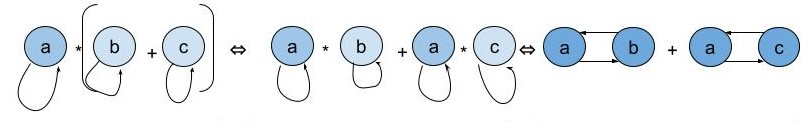
\includegraphics[width=\linewidth]{0226Distributivity.jpg}
  \caption{Associativity of multiplication.}
  \label{fig:0226Distributivity}
\end{figure}

$\\ $

$\textbf{a + b + c}$

$\\ $

$
\begin{matrix}
a = -a & -a = a \\
a \neq -a & -a \neq a\\
\end{matrix}
$

$\\ $

$
\begin{matrix}
b = -b & -b = b \\
b \neq -b & -b \neq b\\
\end{matrix}
$

$\\ $

$
\begin{matrix}
c = -c & -c = c \\
c \neq -c & -c \neq c\\
\end{matrix}
$

$\\ $

$\textbf{a b + a c}$

$\\ $

$
\begin{matrix}
a = -a & -a = a \\
a \neq -a & -a \neq a\\
\end{matrix}
$

$\\ $

$
\begin{matrix}
b = -b & -b = b \\
b \neq -b & -b \neq b\\
\end{matrix}
$

$\\ $

$
\begin{matrix}
a = -a & -a = a \\
a \neq -a & -a \neq a\\
\end{matrix}
$

$\\ $

$
\begin{matrix}
c = -c & -c = c \\
c \neq -c & -c \neq c\\
\end{matrix}
$

$\\ $

$\textbf{a b + a c}$

$\\ $

$
\begin{matrix}
a * b = -a * b & -a * b = a * b\\
a * b \neq -a * b & -a * b \neq a * b\\
\\
b * a = -b*a & -b*a = b * a\\
b * a\neq -b*a & -b*a \neq b * a\\
\\
\\
a * b = b-a & b-a = a * b\\
a * b \neq b-a & b-a \neq a * b\\
\\
b * a = a * -b & -b*a = a * b\\
b * a \neq a * -b & -b*a \neq a * b\\
\end{matrix}
$

$\\ $

$
\begin{matrix}
a * c = -a * c & -a * c = a * c\\
a * c \neq -a * c & -a * c \neq a * c\\
\\
c * a = -c*a & -c*a = c * a\\
c * a\neq -c*a & -c*a \neq c * a\\
\\
\\
a * c = c-a & c-a = a * c\\
a * c \neq c-a & c-a \neq a * c\\
\\
c * a = a * -c & -c*a = a * c\\
c * a \neq a * -c & -c*a \neq a * c\\
\end{matrix}
$

\section{Field}

These rules result in a field defined by Wolfram.

$\\ $

$
\begin{matrix}
Axioms & Addition & Multiplication\\
Commutativity & a+b = b+a & a*b = b*a\\
Identity & a+0 = a = 0+a & a*1 = a = 1*a\\
Inverses & a+(-a)=0=(-a)+a & a*a^-1 = 1 = a^-1*a\ if\ a != 0\\
Associativity & (a+b)+c = a+(b+c) & (a*b)*c = a*(b*c)\\
Distributivity & a*(b+c) = a*b+a*c & (a+b)*c = a*(b+c)
\end{matrix}
$

$\\ $

This field is seen in $\textit{Garg, Gurvits, Oliveira, and Wigderson}$. 

$\\ $

Using this result, a more formal definition of an inferrable language can be derived in order to find more mathematical relationships.

$\\ $

$\textit{Definition}$. An inferrable language, $L$, is a set of at least two sequences where each sequence satisfies a linear recurrence relation that forms a ring. Equivalently, given $A_i \in L$ for any $i \leq n$ where $A_i = a_i - \sum_{k \neq i}a_k = 0$ implies $a_i = \sum_{k \neq i}a_k$ then $a_i = \sum_{k \neq i}a_k$ thus a decision function is equivalent to $a_i = \sum_{j \neq i}A_j + \sum_{k \neq i}a_k$.

$\\ $

$\textit{Definition}$. A decision function on an inferrable language is a linear recurrence relation where at least two sequences in the language are combined to form a relation for any of the chosen sequence.

$\\ $

There exists an equivalent relation in regards to the rational series describing semigroup monoids in the following definition.

$\\ $

$\textit{Definition}$. An inferrable language consists of at least two ideals containing elements such that for every element in the ideal each element has a morphism that contains elements other than itself in the ideal, $I_1$, and at least one other ideal, $I_2$. Equivalently, given $I_i$ such that $i \leq i \leq n$ where $I_i = (S_i, P)$ and $m_k \in (S_i, P)$ then $m_k = \sum_{j \neq k}(S_j, P) + \sum_{l \neq i}I_l$ called the decision function.

$\\ $

$\textit{Definition}$. A decider is the set of all decision functions on each element for at least two ideals such that $m = f(x) \in I$.

$\\ $
%\include{Chapters/Chapter4} 
%\include{Chapters/Chapter5} 

%----------------------------------------------------------------------------------------
%	THESIS CONTENT - APPENDICES
%----------------------------------------------------------------------------------------

% Include the appendices of the thesis as separate files from the Appendices folder
% Uncomment the lines as you write the Appendices

%% Appendix A

\chapter{Frequently Asked Questions} % Main appendix title

\label{AppendixA} % For referencing this appendix elsewhere, use \ref{AppendixA}

\section{How do I change the colors of links?}

The color of links can be changed to your liking using:

{\small\verb!\hypersetup{urlcolor=red}!}, or

{\small\verb!\hypersetup{citecolor=green}!}, or

{\small\verb!\hypersetup{allcolor=blue}!}.

\noindent If you want to completely hide the links, you can use:

{\small\verb!\hypersetup{allcolors=.}!}, or even better: 

{\small\verb!\hypersetup{hidelinks}!}.

\noindent If you want to have obvious links in the PDF but not the printed text, use:

{\small\verb!\hypersetup{colorlinks=false}!}.

%\include{Appendices/AppendixB}
%\include{Appendices/AppendixC}

%----------------------------------------------------------------------------------------
%	BIBLIOGRAPHY
%----------------------------------------------------------------------------------------


\chapter{References} % Main appendix title

$\\ $

Valiant, Leslie., Holographic Algorithms.

Berstel, J., \& Reutenauer, C. (2010). Noncommutative rational series with applications. Cambridge University Press.

Sipser, M. (2006). Theory of Computation (2nd ed., p. 431). Course Technology, Cengage Learning.

Munkres, J. R. (2000). Topology (2nd ed., p. 537). Prentice Hall.

Artin, M. (2011). Algebra (2nd ed., p. 543). Pearson.

Enderton, H. B. (2001). Logic (2nd ed., p. 317). HARCOURT/ACADEMIC PRESS.

Lay, S. R. (2004). Analysis (4th ed., p. 394). Pearson Prentice Hall.

Cox, D. A., Little, J., \& O’Shea, D. (1997). Ideals, varieties, and algorithms: An introduction to computational algebraic geometry and commutative algebra (2nd ed.). Springer.

Golub, G. H., \& Van Loan, C. F. (1996). Matrix Computations (3rd ed., p. 728). Johns Hopkins University Press.

Hofstadter, D. R. (1999). Gödel, Escher, Bach: An eternal golden braid. Basic Books.

Cormen, T. H., Leiserson, C. E., Rivest, R. L., \& Stein, C. (2009). Introduction to Algorithms (3rd ed.). MIT Press.

Shilov, G. E. (2012). Linear algebra (R. A. Silverman, Trans.). Dover Publications. (Original work published 1971)

Strang, G. (2009). Introduction to Linear Algebra (4th ed., p. 585). Wellesley-Cambridge Press.

Rosen, K. H. (2006). Discrete Mathematics And Its Applications (6th ed.). McGraw-Hill Education.

Prasolov, V. V. (1995). Intuitive topology. American Mathematical Society.

Carter, N. (2009). Visual group theory. Mathematical Association of America.

Spivak, M. (2008). Calculus (4th ed., p. 680). Publish or Perish.

Sullivan, M. (2008). Precalculus (8th ed., p. 1152). Prentice Hall.

Ung, E. (2023). A Language of Polynomials (Version 1.0.0). 

Hamming, R. W. (1986). Numerical methods for scientists and engineers. Courier Corporation.

Weisstein, Eric W. "Field Axioms." From MathWorld--A Wolfram Web Resource. 

Pinter, C. C. (2010). A book of abstract algebra (2nd ed.). Dover Publications.

Ung, E. (2023). Applications For Monomial Deciders (Version 1.0.1).

Ung, E. (2023). A Language Of Polynomials (Version 1.0.1).

Ung, E. (2018). Inferring Lindenmayer Systems.




%----------------------------------------------------------------------------------------

\end{document}  
